\begin{frame}[c]
    \frametitle{Agenda}
    \begin{itemize}
        \item Overview
        \begin{itemize}
            \item Markov Chains \& Stepsizes
            \item Effectiveness \& Expected Squared Jump Distance 
            \item Thompson Sampling
            \item Once more: Why not to tune the acceptance rate!
        \end{itemize}
        \item Results
        \item Improvements \& More
        \begin{itemize}
            \item Acceptance Rate Tuning with Thompson Sampling
            \item Tune higher-order Autocorrelation Lags
            \item Gaussian Process Time Costs
            \item Monotonicity of Thinning
        \end{itemize}
    \end{itemize}
\end{frame}

\begin{frame}[c]
    \frametitle{Agenda}
    \begin{itemize}
        \item Overview
        \begin{itemize}
            \item Markov Chains \& Stepsizes
            {\color{lgray}
            \item Effectiveness \& Expected Squared Jump Distance 
            \item Thompson Sampling
            \item Once more: Why not to tune the acceptance rate!
            }
        \end{itemize}
        {\color{lgray}
        \item Results
        \item Improvements \& More
        }
        \begin{itemize}
            {\color{lgray}
            \item Acceptance Rate Tuning with Thompson Sampling
            \item Tune higher-order Autocorrelation Lags
            \item Gaussian Process Time Costs
            \item Monotonicity of Thinning
        }
        \end{itemize}
    \end{itemize}
\end{frame}

\begin{frame}[c]
    \frametitle{Markov Chains ...}
    \begin{itemize}
        \item A Markov chain is a stochastic process $X_0, X_1, \ldots$ which takes values from some 
            state space $\Theta$ and where the following properties hold:\vspace{.2cm}
            \begin{itemize}
                \item $ \displaystyle \mathbb{P}(X_{0} = \theta_{0}) = \lambda(\theta_0)$ \vspace{.2cm}
                \item $ \displaystyle
                    \mathbb{P}(X_{t+1} = \theta_{t+1} | X_t = \theta_t , \ldots, X_0 = \theta_0) 
                    = \mathbb{P}(X_{t+1} = \theta_{t+1} | X_t = \theta_t) =: P(\theta_t, \theta_{t+1}) $\vspace{.2cm}
        \end{itemize}
        where $\lambda$ is a distribution over $\Theta$
        \item[] \vspace{-.3cm}
        \item An example: $\Theta = [0, 3]\cap \mathbb{N}$ and $P = \begin{pmatrix} p & p & & \\ p &  & p & \\ & p & & p \\ & & p & p \end{pmatrix}$ with $p = 0.5$
    \end{itemize}
    \vspace{-0.5cm}
    \begin{center}
        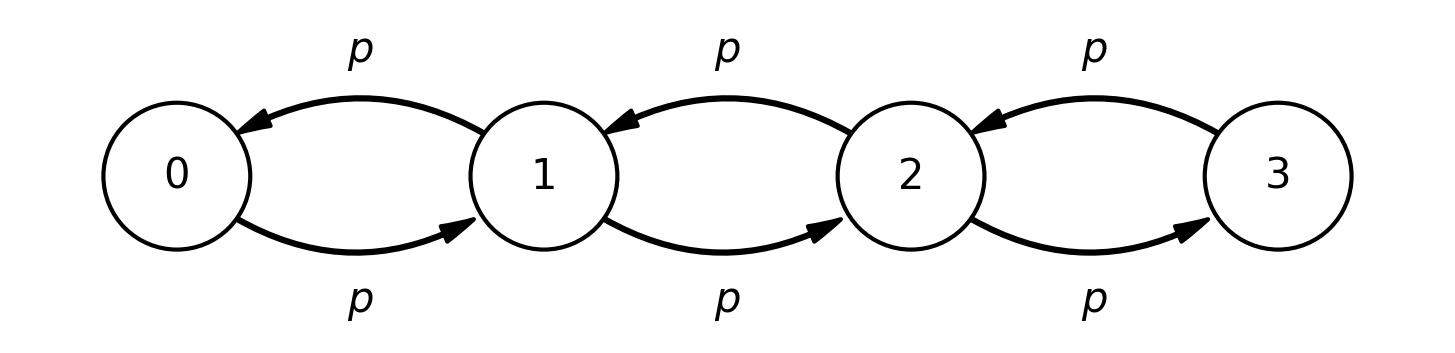
\includegraphics[scale=0.8]{imgs/uniformchain.png}
    \end{center}
\end{frame}

\begin{frame}[c]
    \frametitle{Markov Chains ...}
    \begin{itemize}
        \item We simulate and count ...
    \end{itemize}
    \begin{center}
        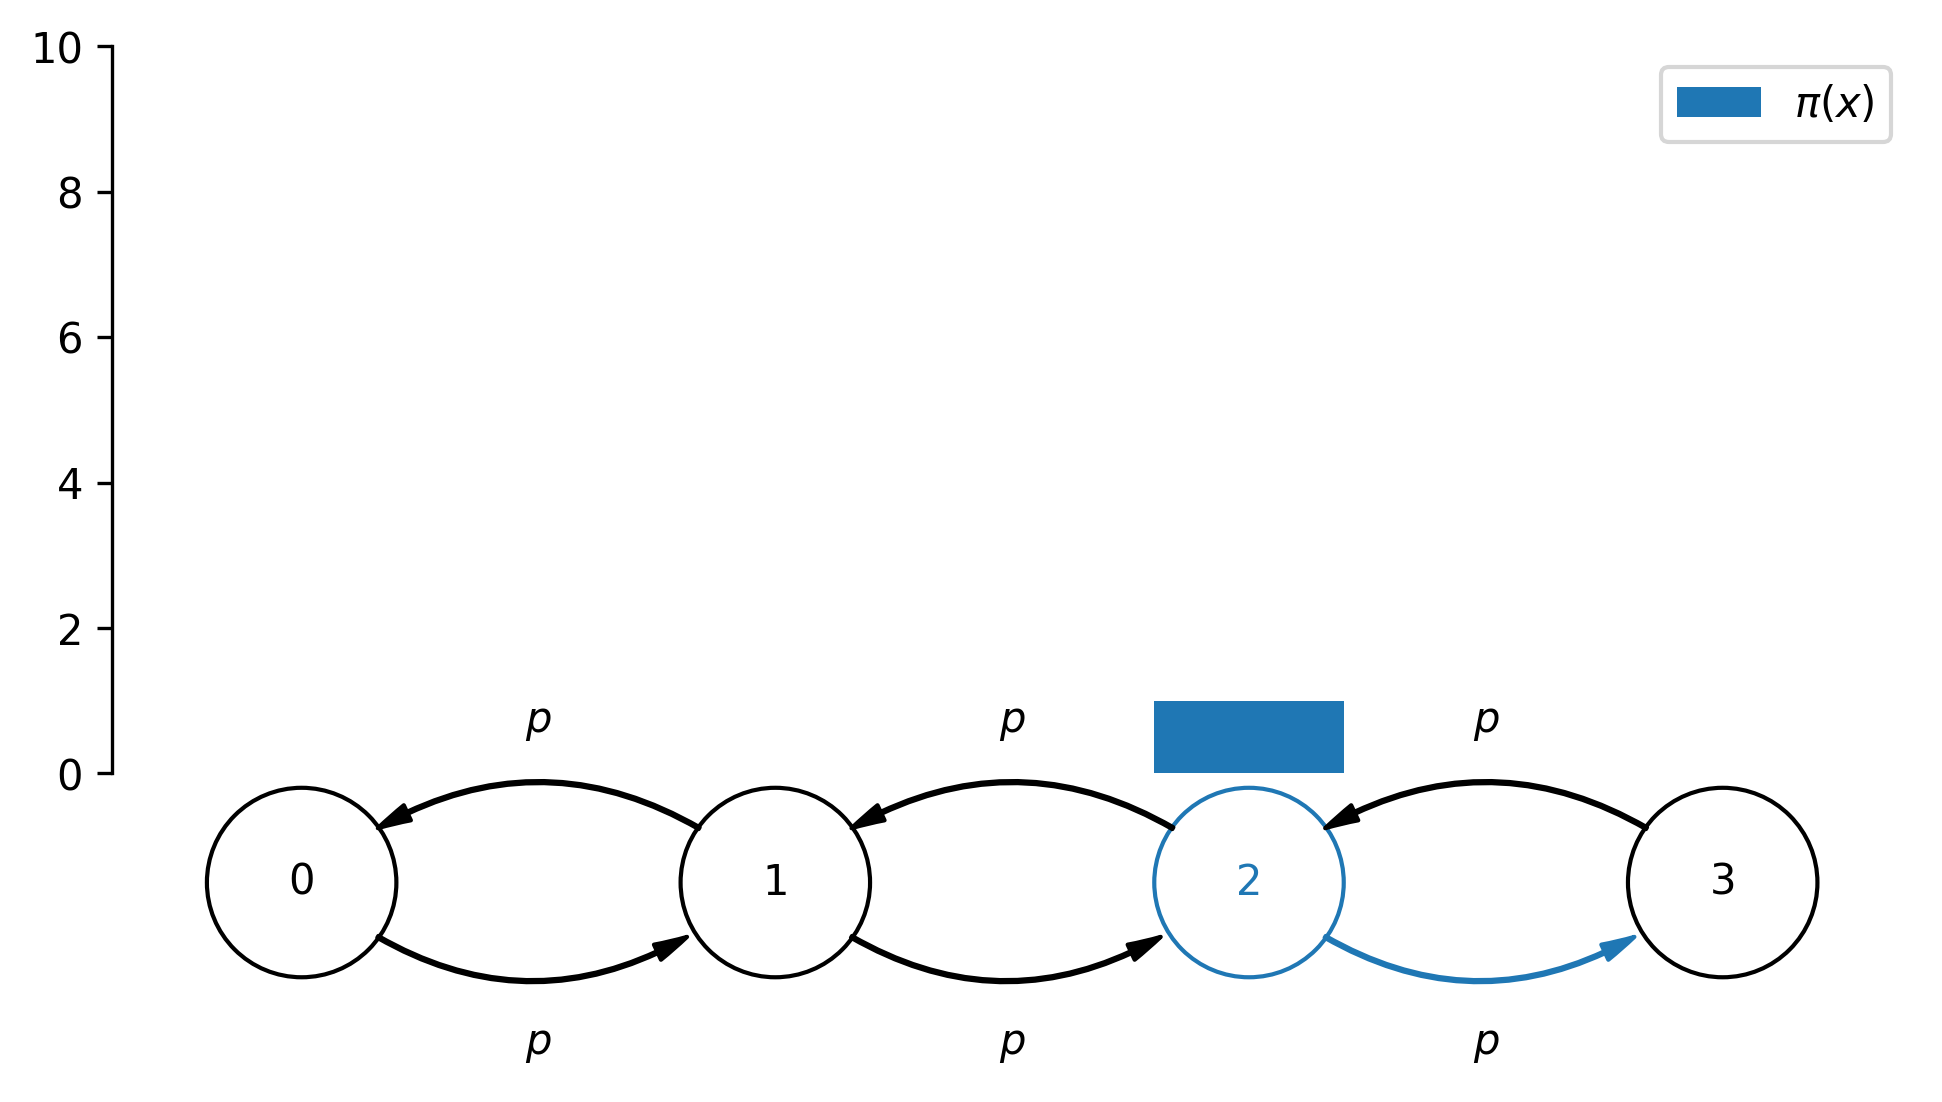
\includegraphics[scale=0.6]{imgs/simulation0.png}
    \end{center}
\end{frame}

\begin{frame}[c]
    \frametitle{Markov Chains ...}
    \begin{itemize}
        \item We simulate and count ...
    \end{itemize}
    \begin{center}
        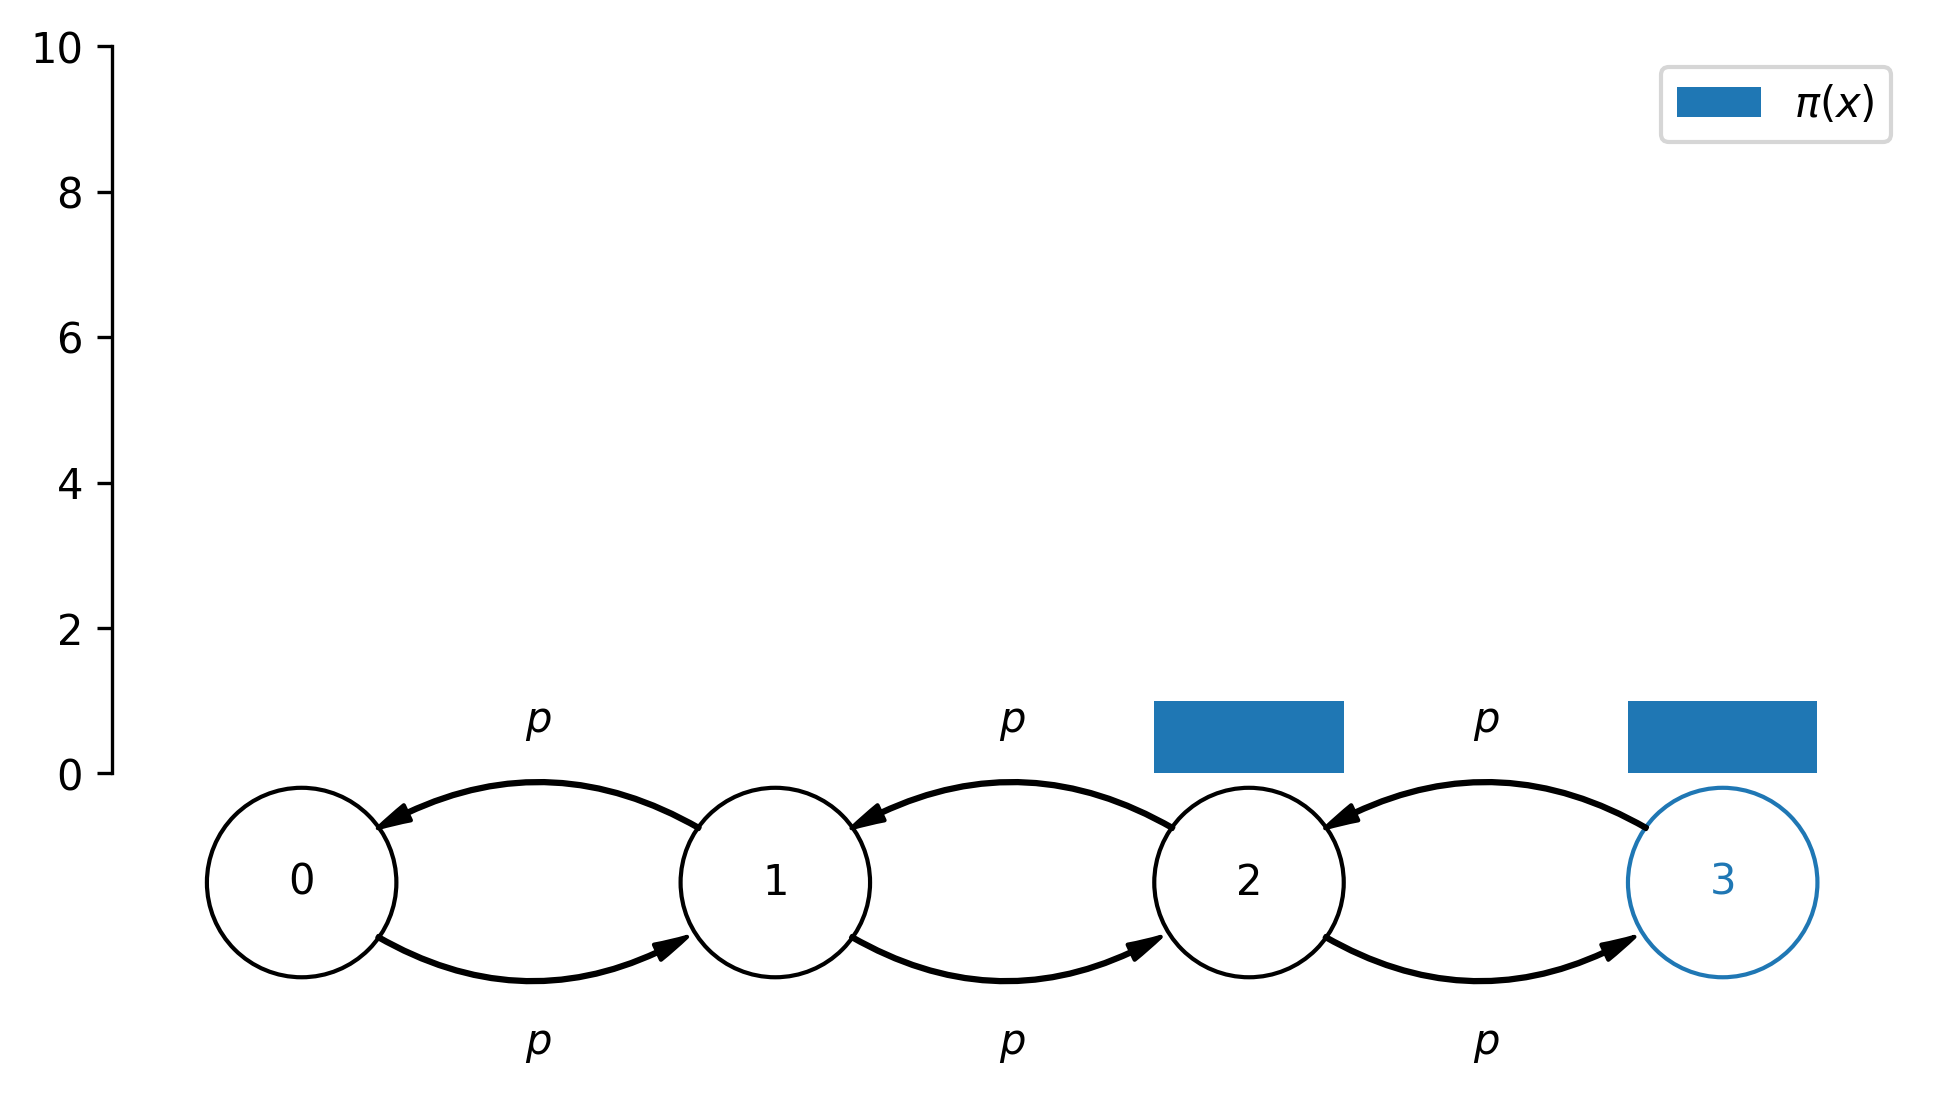
\includegraphics[scale=0.6]{imgs/simulation1.png}
    \end{center}
\end{frame}

\begin{frame}[c]
    \frametitle{Markov Chains ...}
    \begin{itemize}
        \item We simulate and count ...
    \end{itemize}
    \begin{center}
        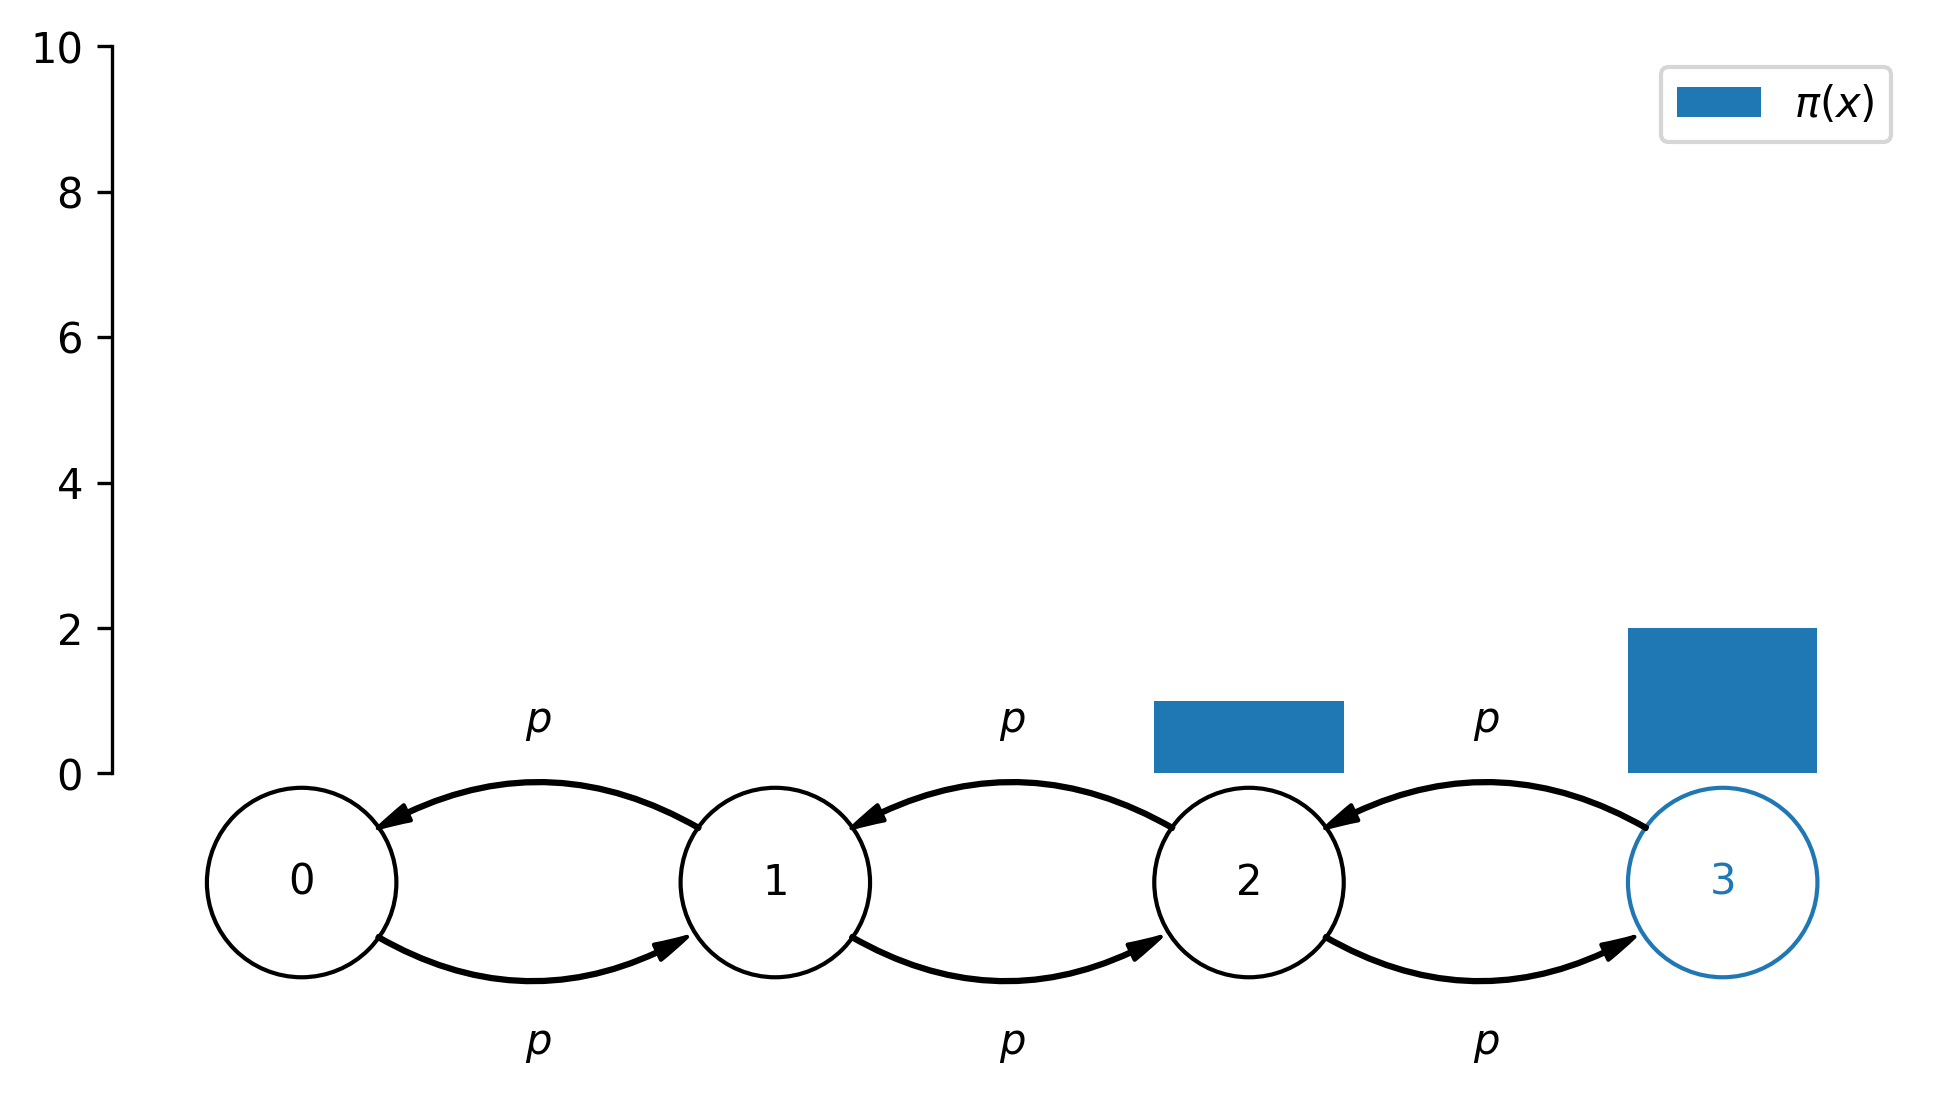
\includegraphics[scale=0.6]{imgs/simulation2.png}
    \end{center}
\end{frame}

\begin{frame}[c]
    \frametitle{Markov Chains ...}
    \begin{itemize}
        \item We simulate and count ...
    \end{itemize}
    \begin{center}
        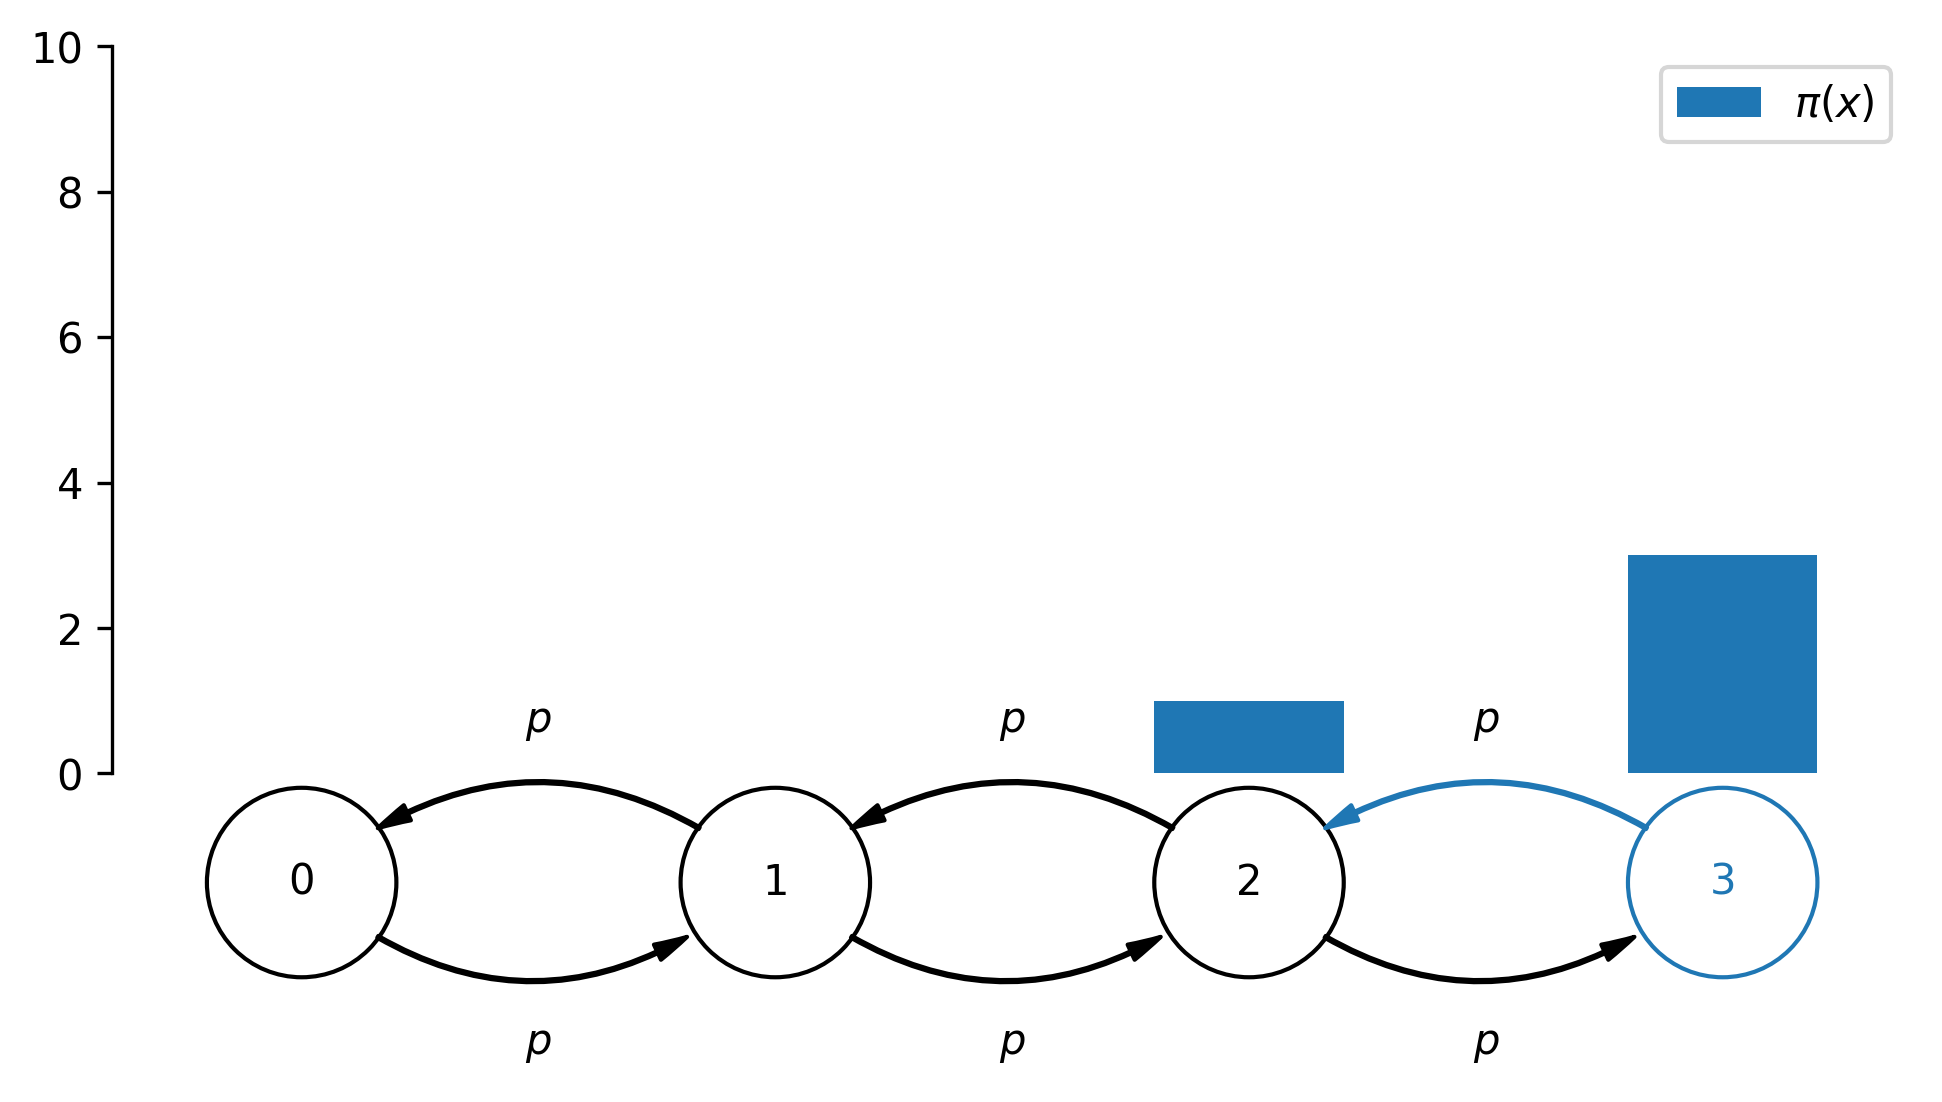
\includegraphics[scale=0.6]{imgs/simulation3.png}
    \end{center}
\end{frame}

\begin{frame}[c]
    \frametitle{Markov Chains ...}
    \begin{itemize}
        \item We simulate and count ...
    \end{itemize}
    \begin{center}
        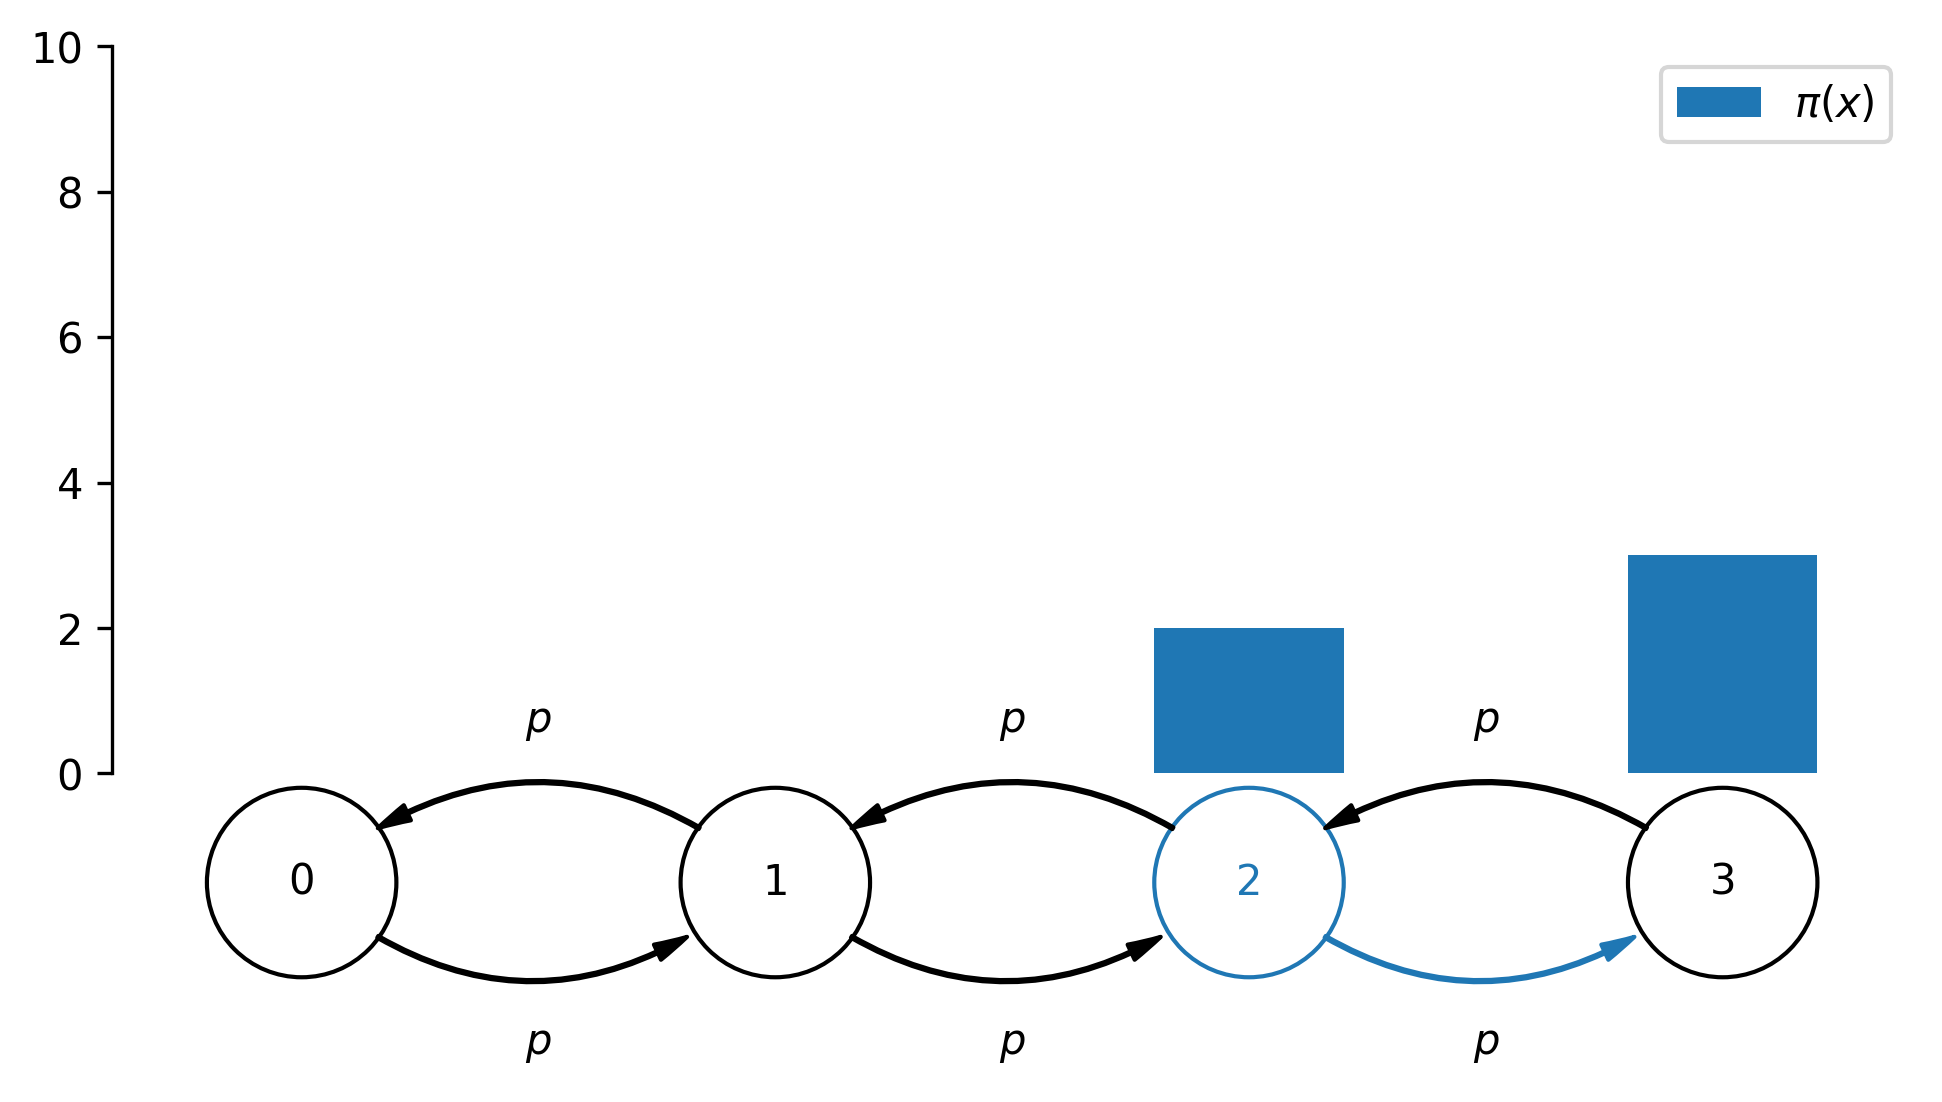
\includegraphics[scale=0.6]{imgs/simulation4.png}
    \end{center}
\end{frame}

\begin{frame}[c]
    \frametitle{Markov Chains ...}
    \begin{itemize}
        \item We simulate and count ...
    \end{itemize}
    \begin{center}
        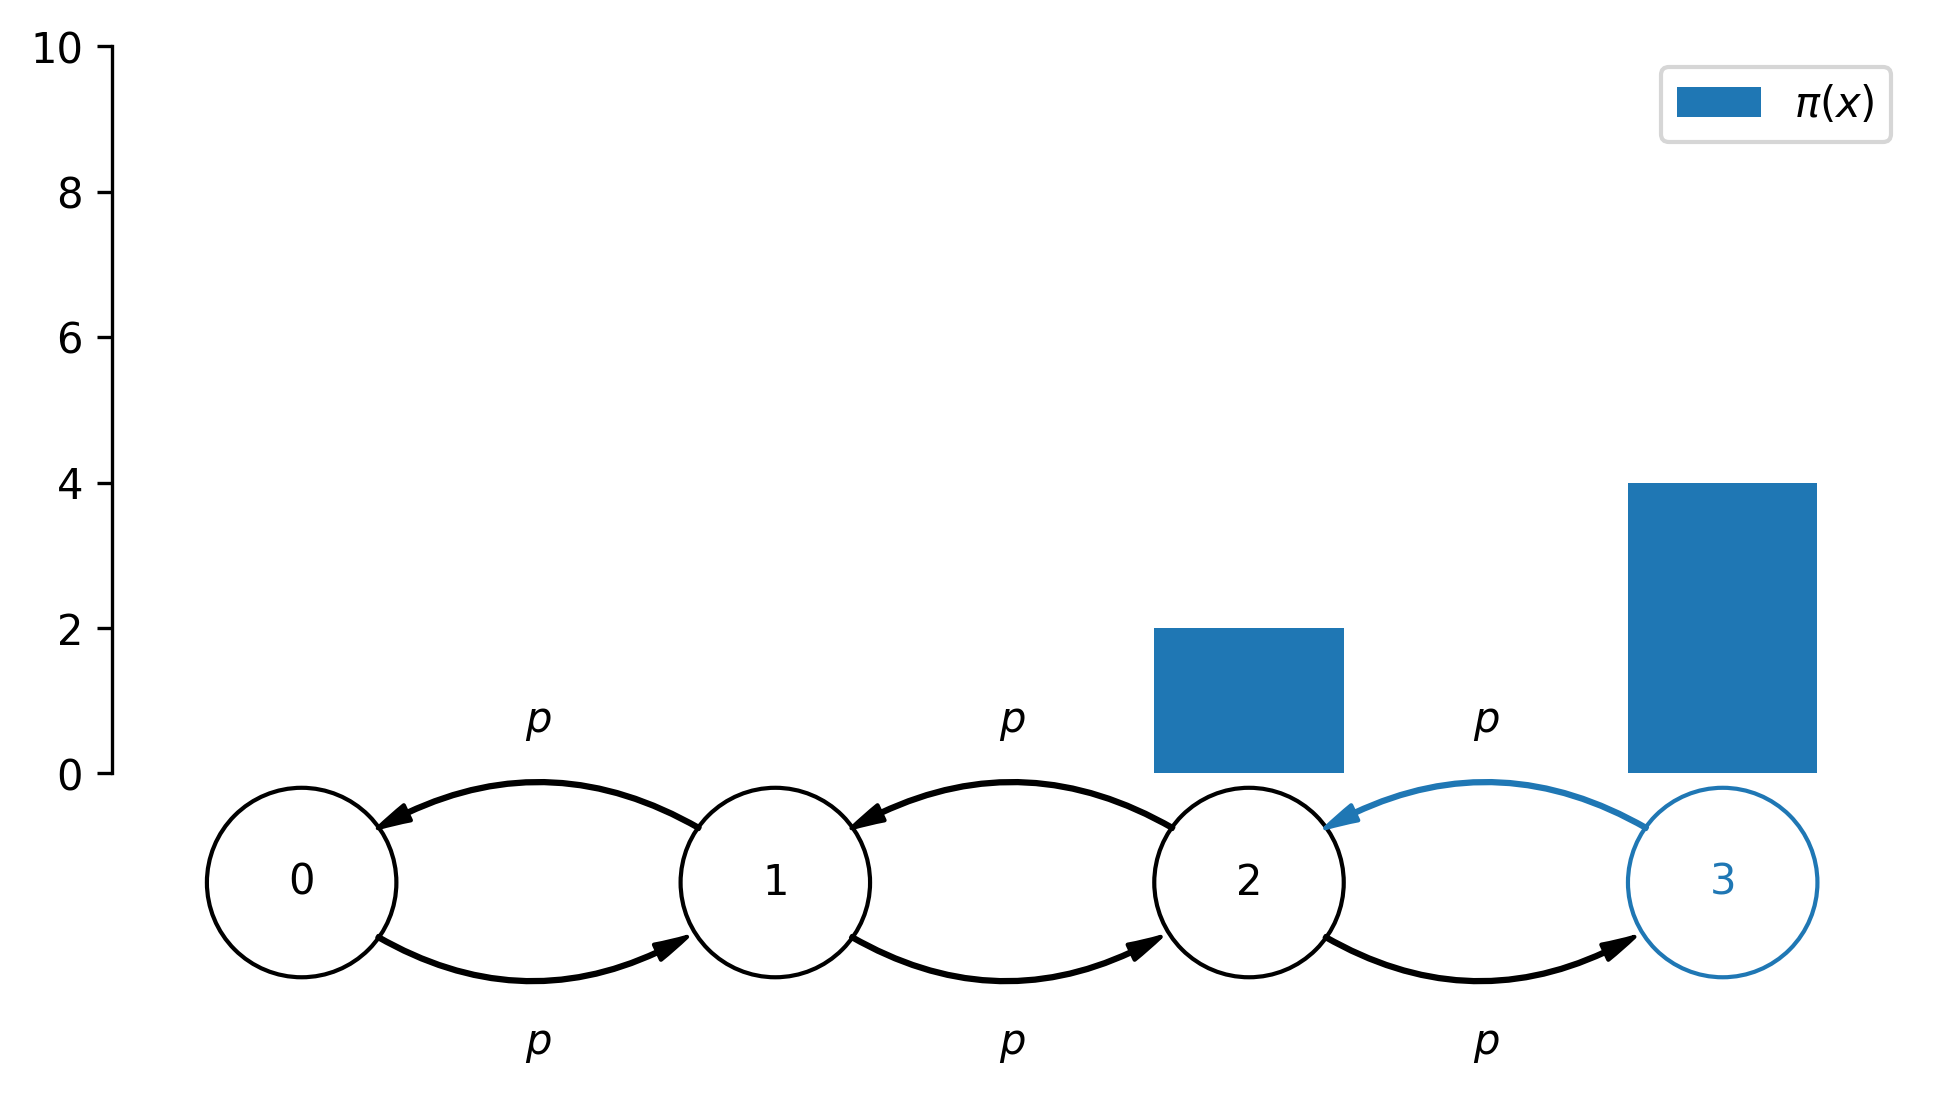
\includegraphics[scale=0.6]{imgs/simulation5.png}
    \end{center}
\end{frame}

\begin{frame}[c]
    \frametitle{Markov Chains ...}
    \begin{itemize}
        \item We simulate and count ...
    \end{itemize}
    \begin{center}
        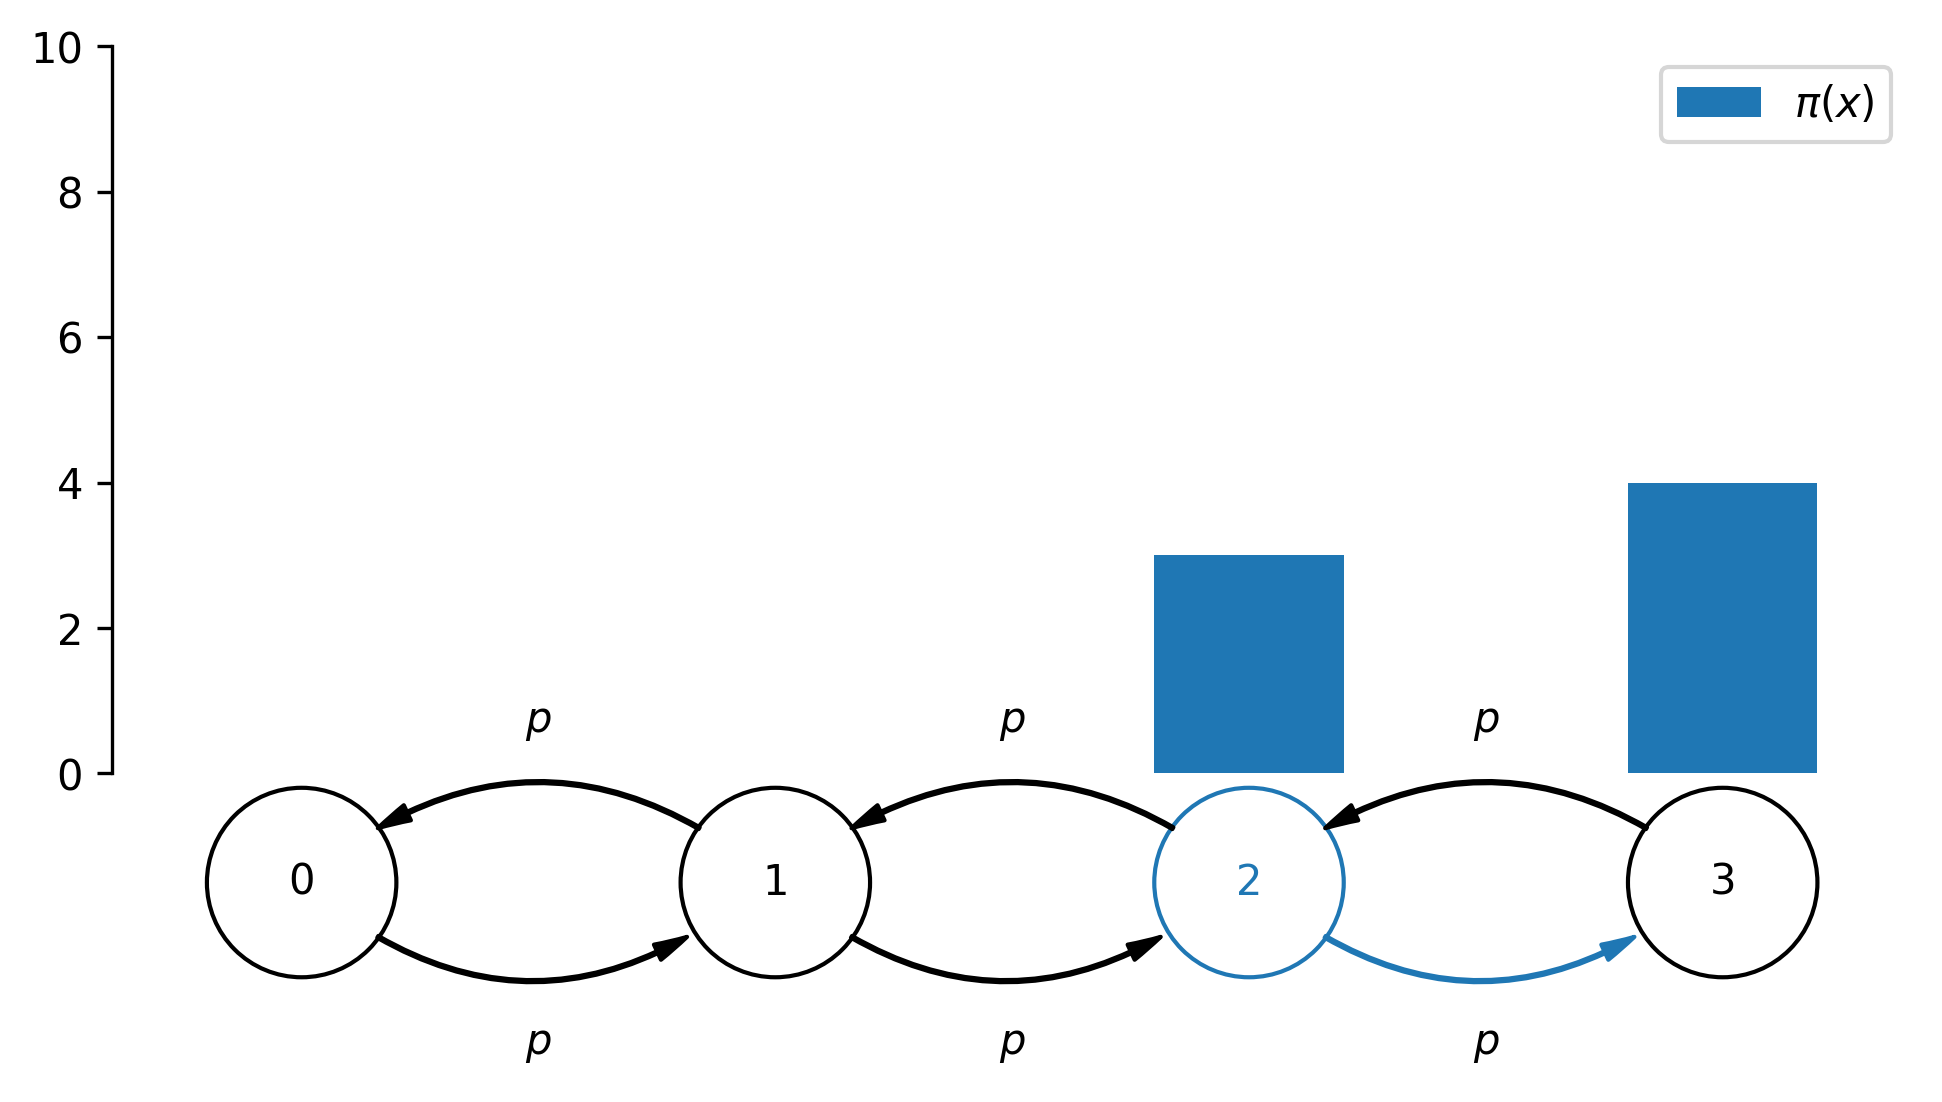
\includegraphics[scale=0.6]{imgs/simulation6.png}
    \end{center}
\end{frame}

\begin{frame}[c]
    \frametitle{Markov Chains ...}
    \begin{itemize}
        \item We simulate and count ...
    \end{itemize}
    \begin{center}
        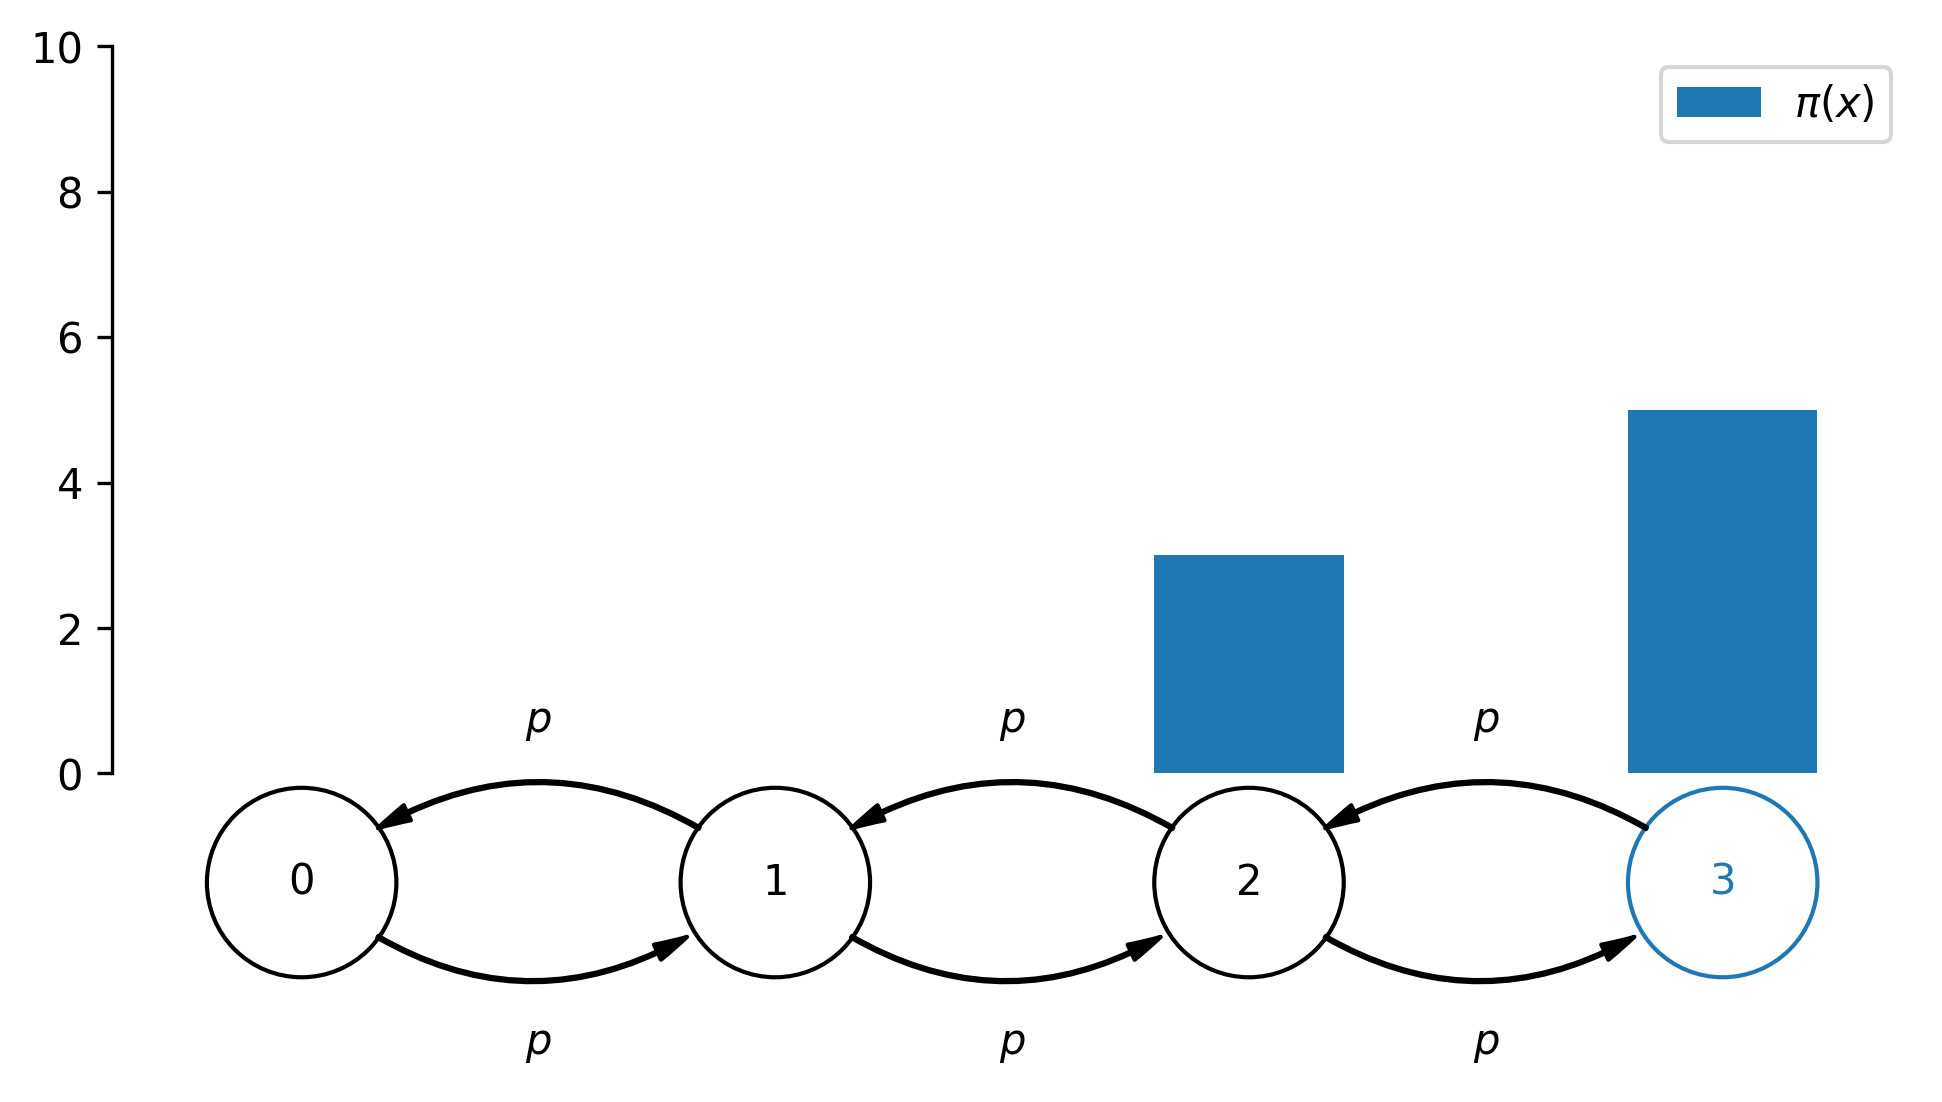
\includegraphics[scale=0.6]{imgs/simulation7.png}
    \end{center}
\end{frame}

\begin{frame}[c]
    \frametitle{Markov Chains ...}
    \begin{itemize}
        \item We simulate and count ...
    \end{itemize}
    \begin{center}
        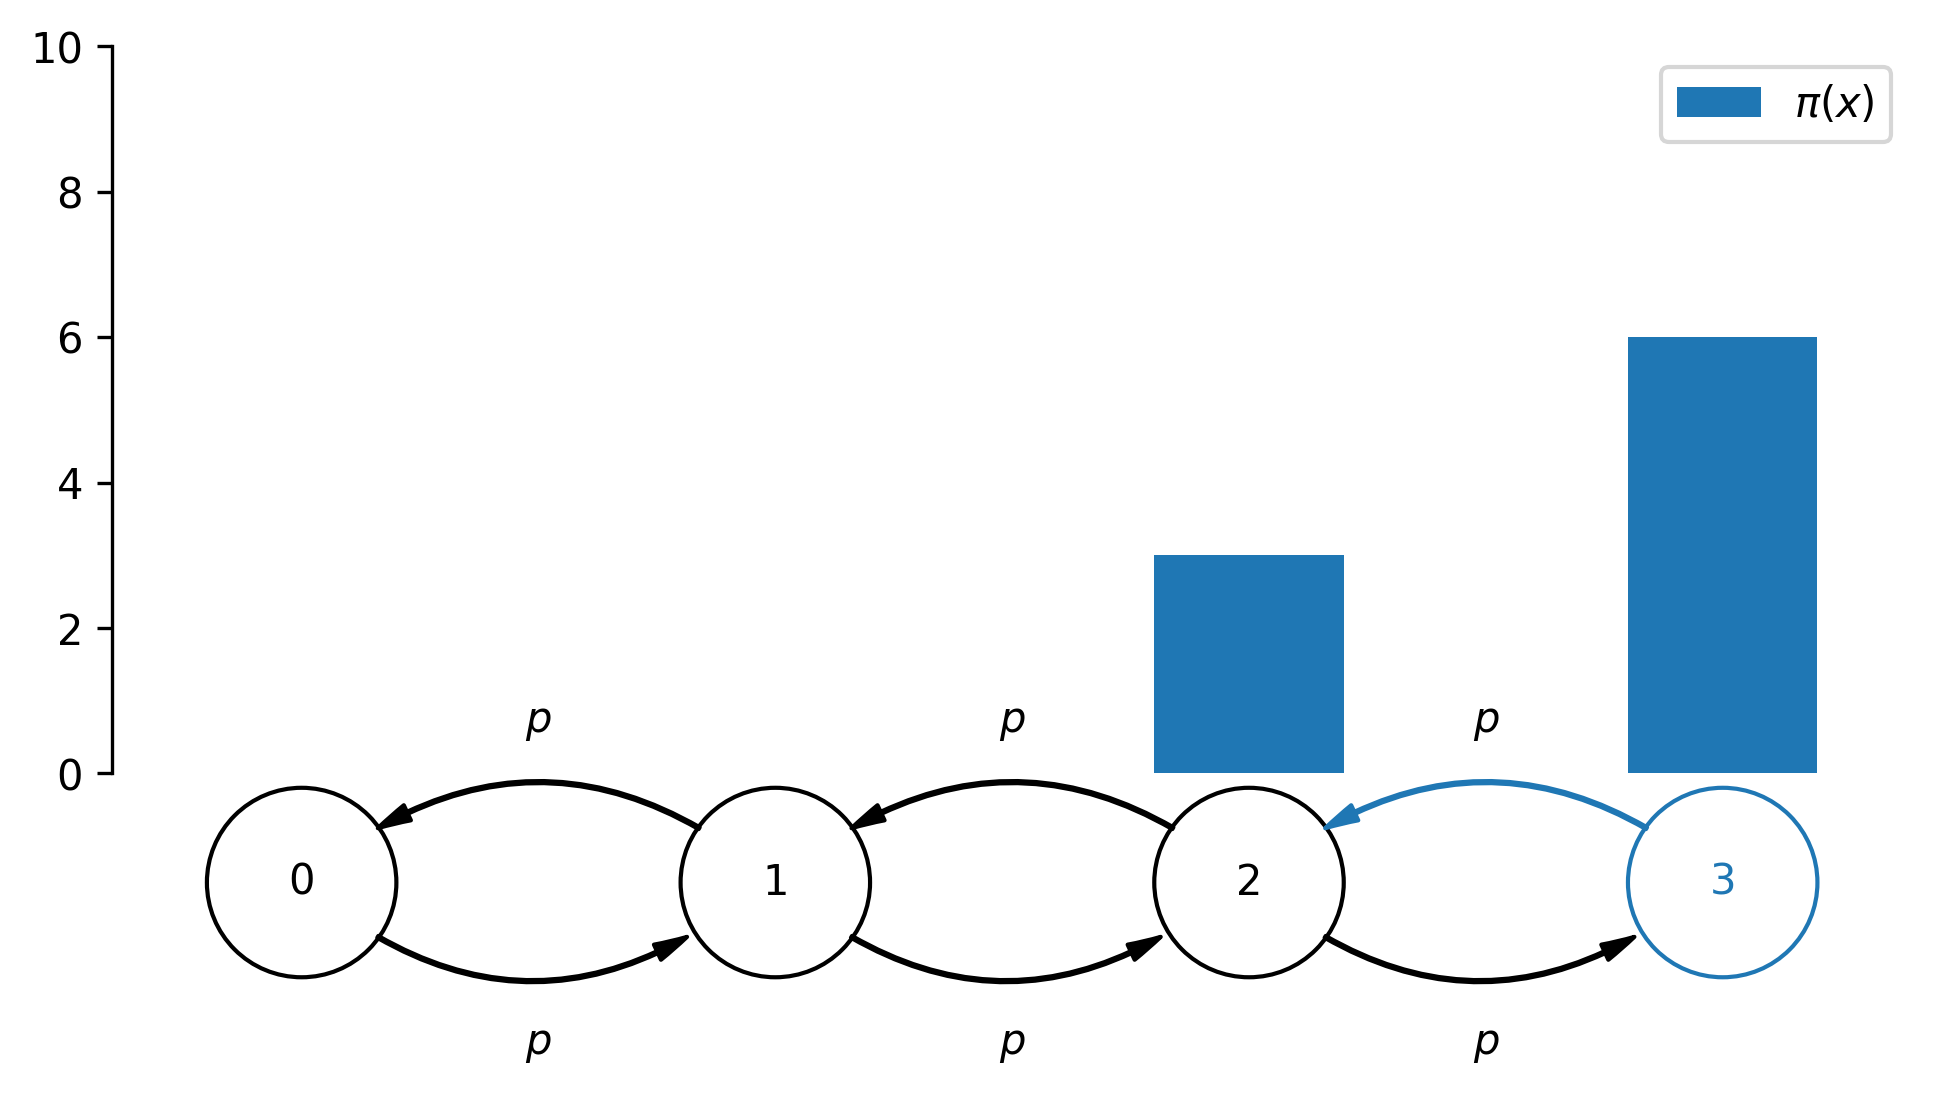
\includegraphics[scale=0.6]{imgs/simulation8.png}
    \end{center}
\end{frame}

\begin{frame}[c]
    \frametitle{Markov Chains ...}
    \begin{itemize}
        \item We simulate and count ...
    \end{itemize}
    \begin{center}
        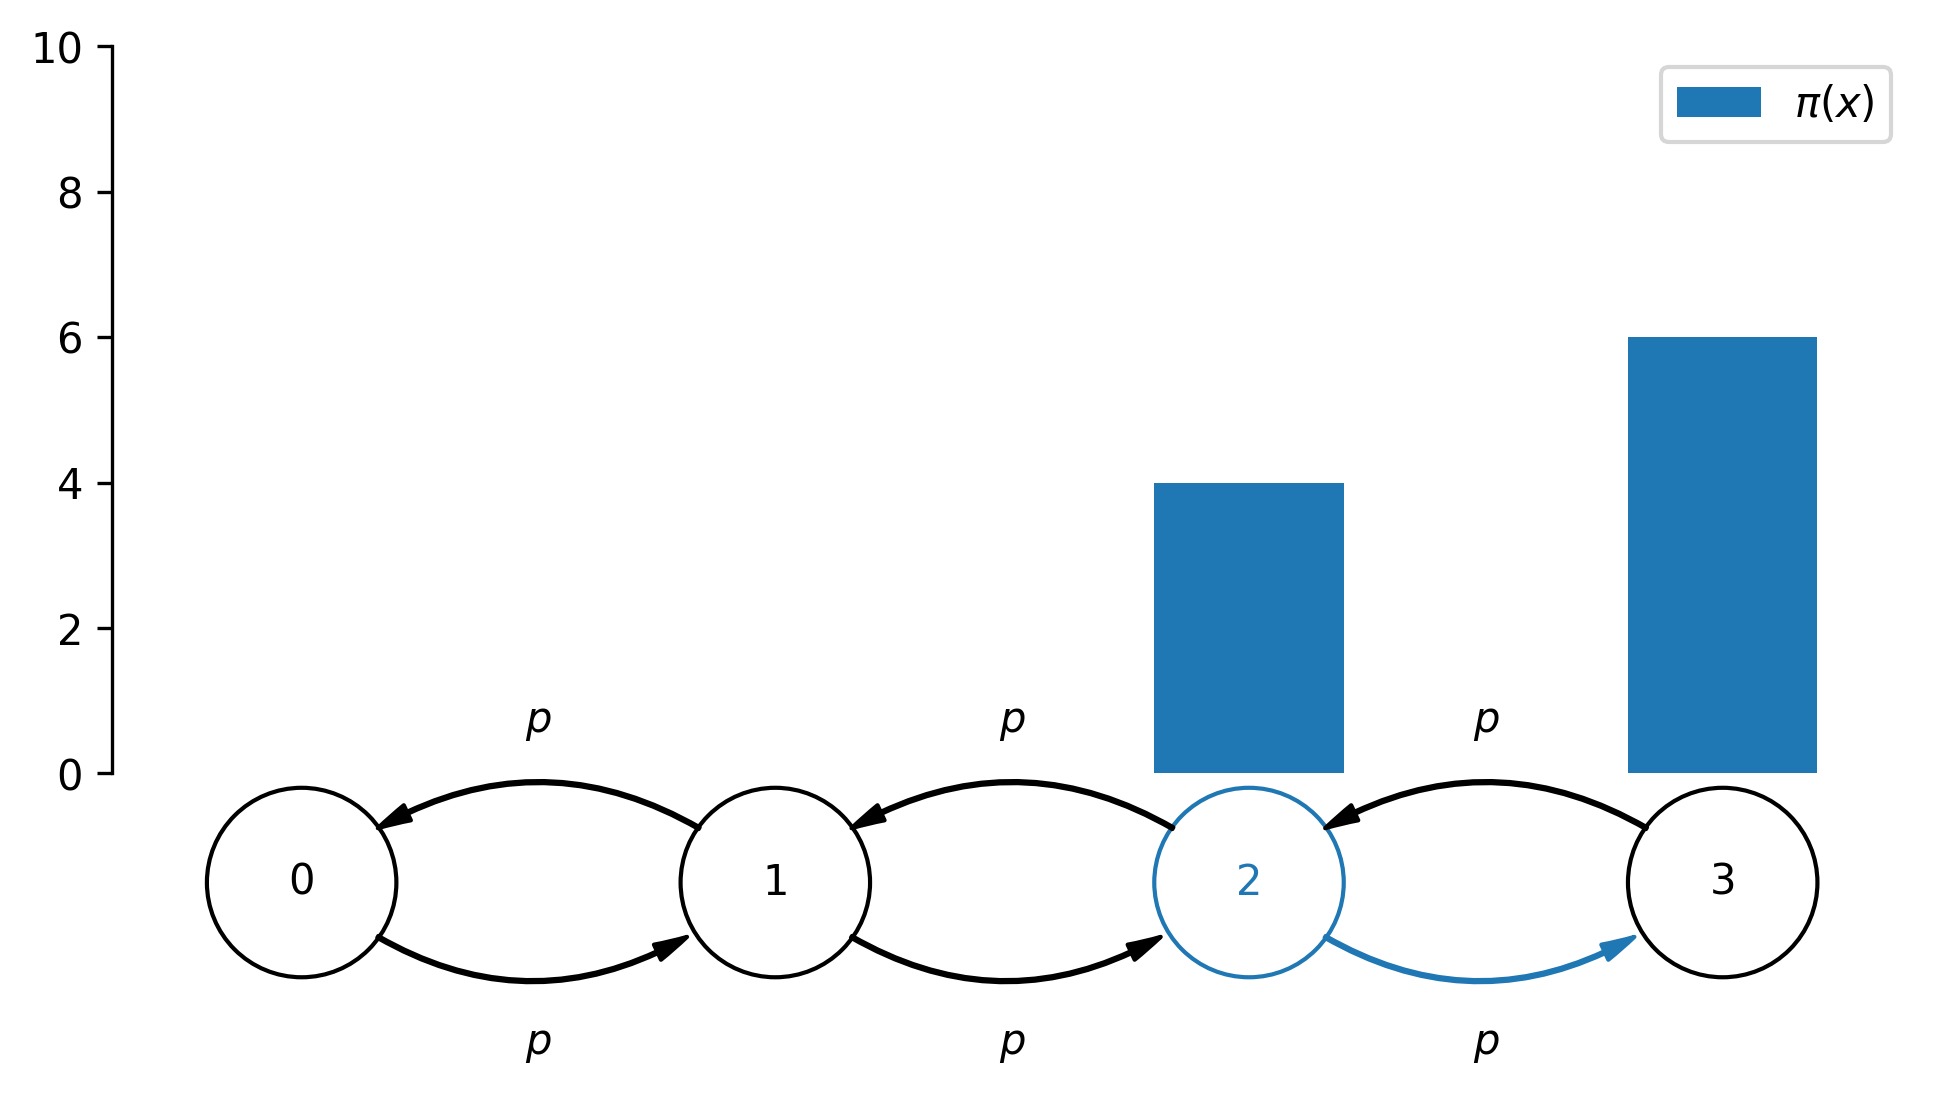
\includegraphics[scale=0.6]{imgs/simulation9.png}
    \end{center}
\end{frame}

\begin{frame}[c]
    \frametitle{Markov Chains ...}
    \begin{itemize}
        \item We simulate and count ...
    \end{itemize}
    \begin{center}
        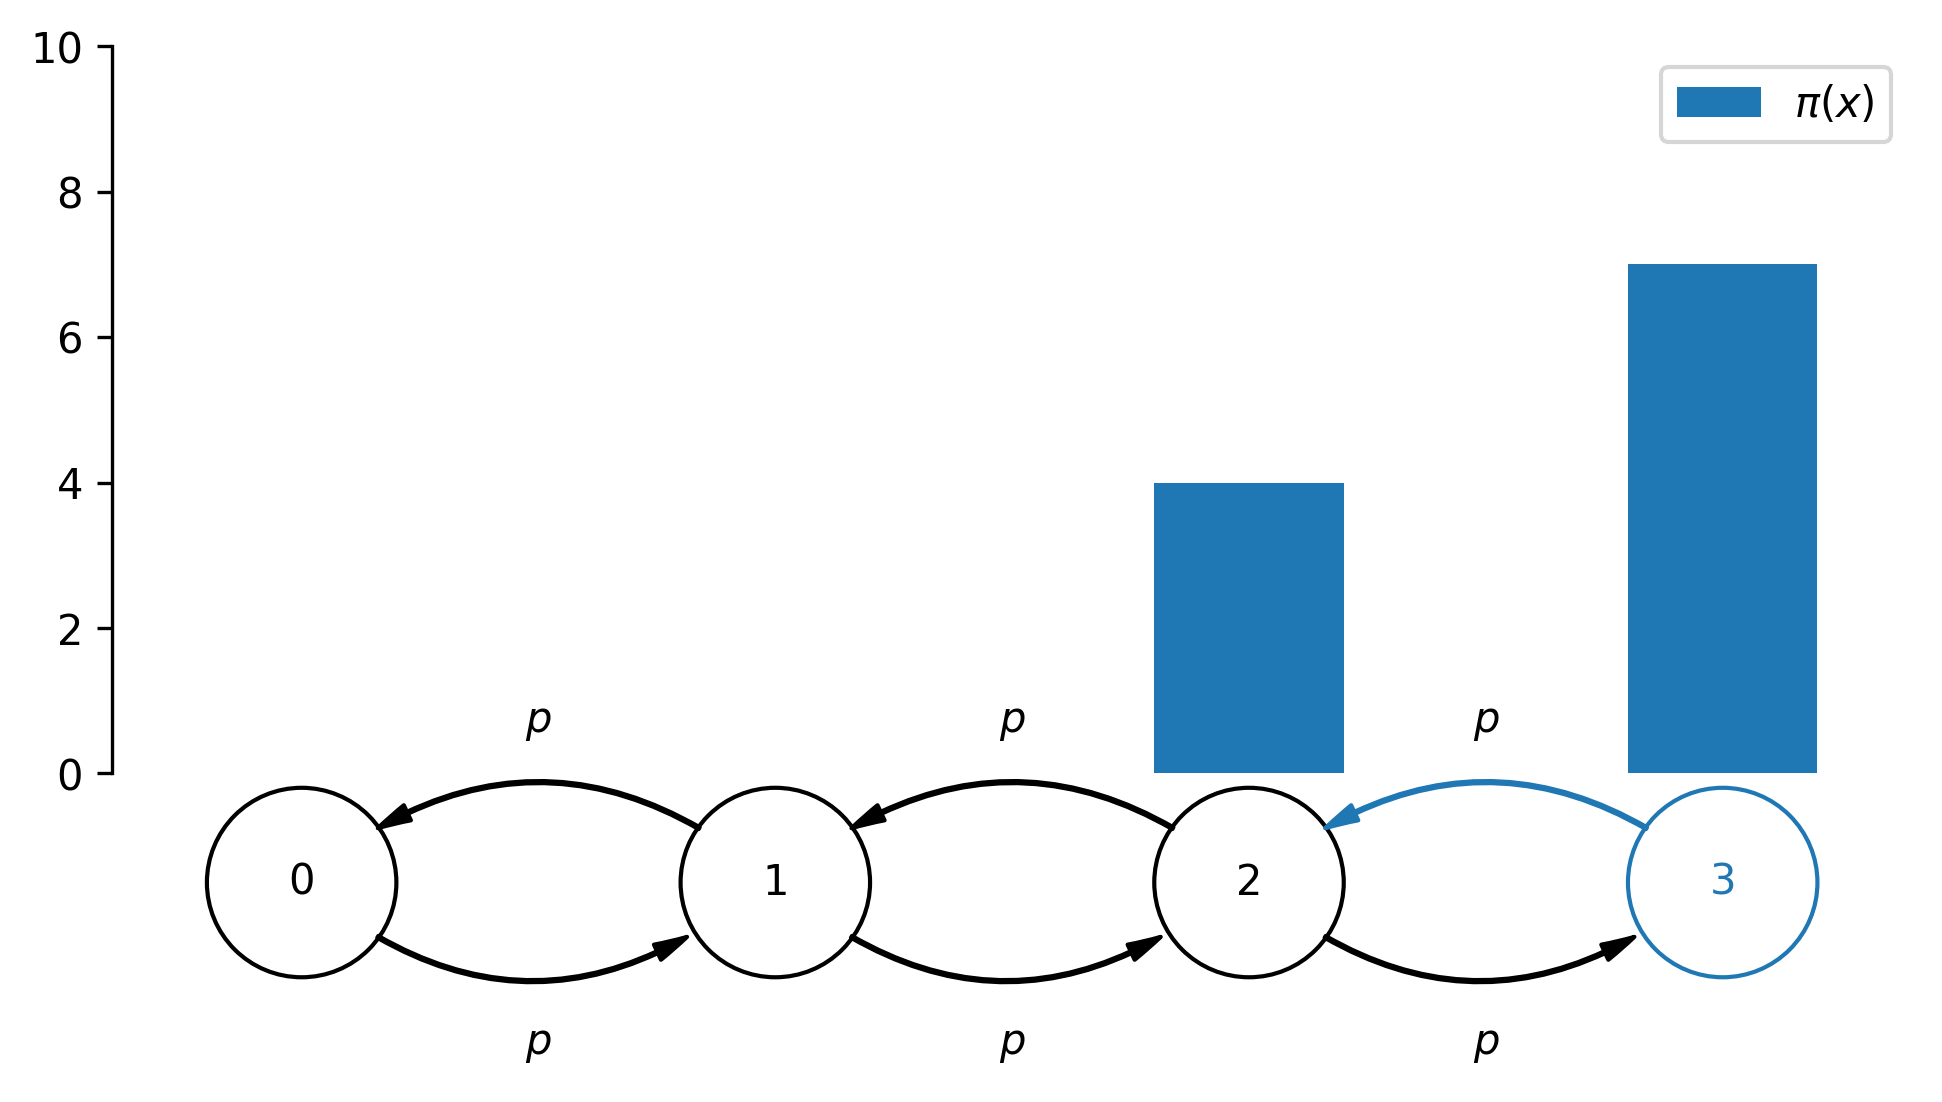
\includegraphics[scale=0.6]{imgs/simulation10.png}
    \end{center}
\end{frame}

\begin{frame}[c]
    \frametitle{Markov Chains ...}
    \begin{itemize}
        \item We simulate and count ...
    \end{itemize}
    \begin{center}
        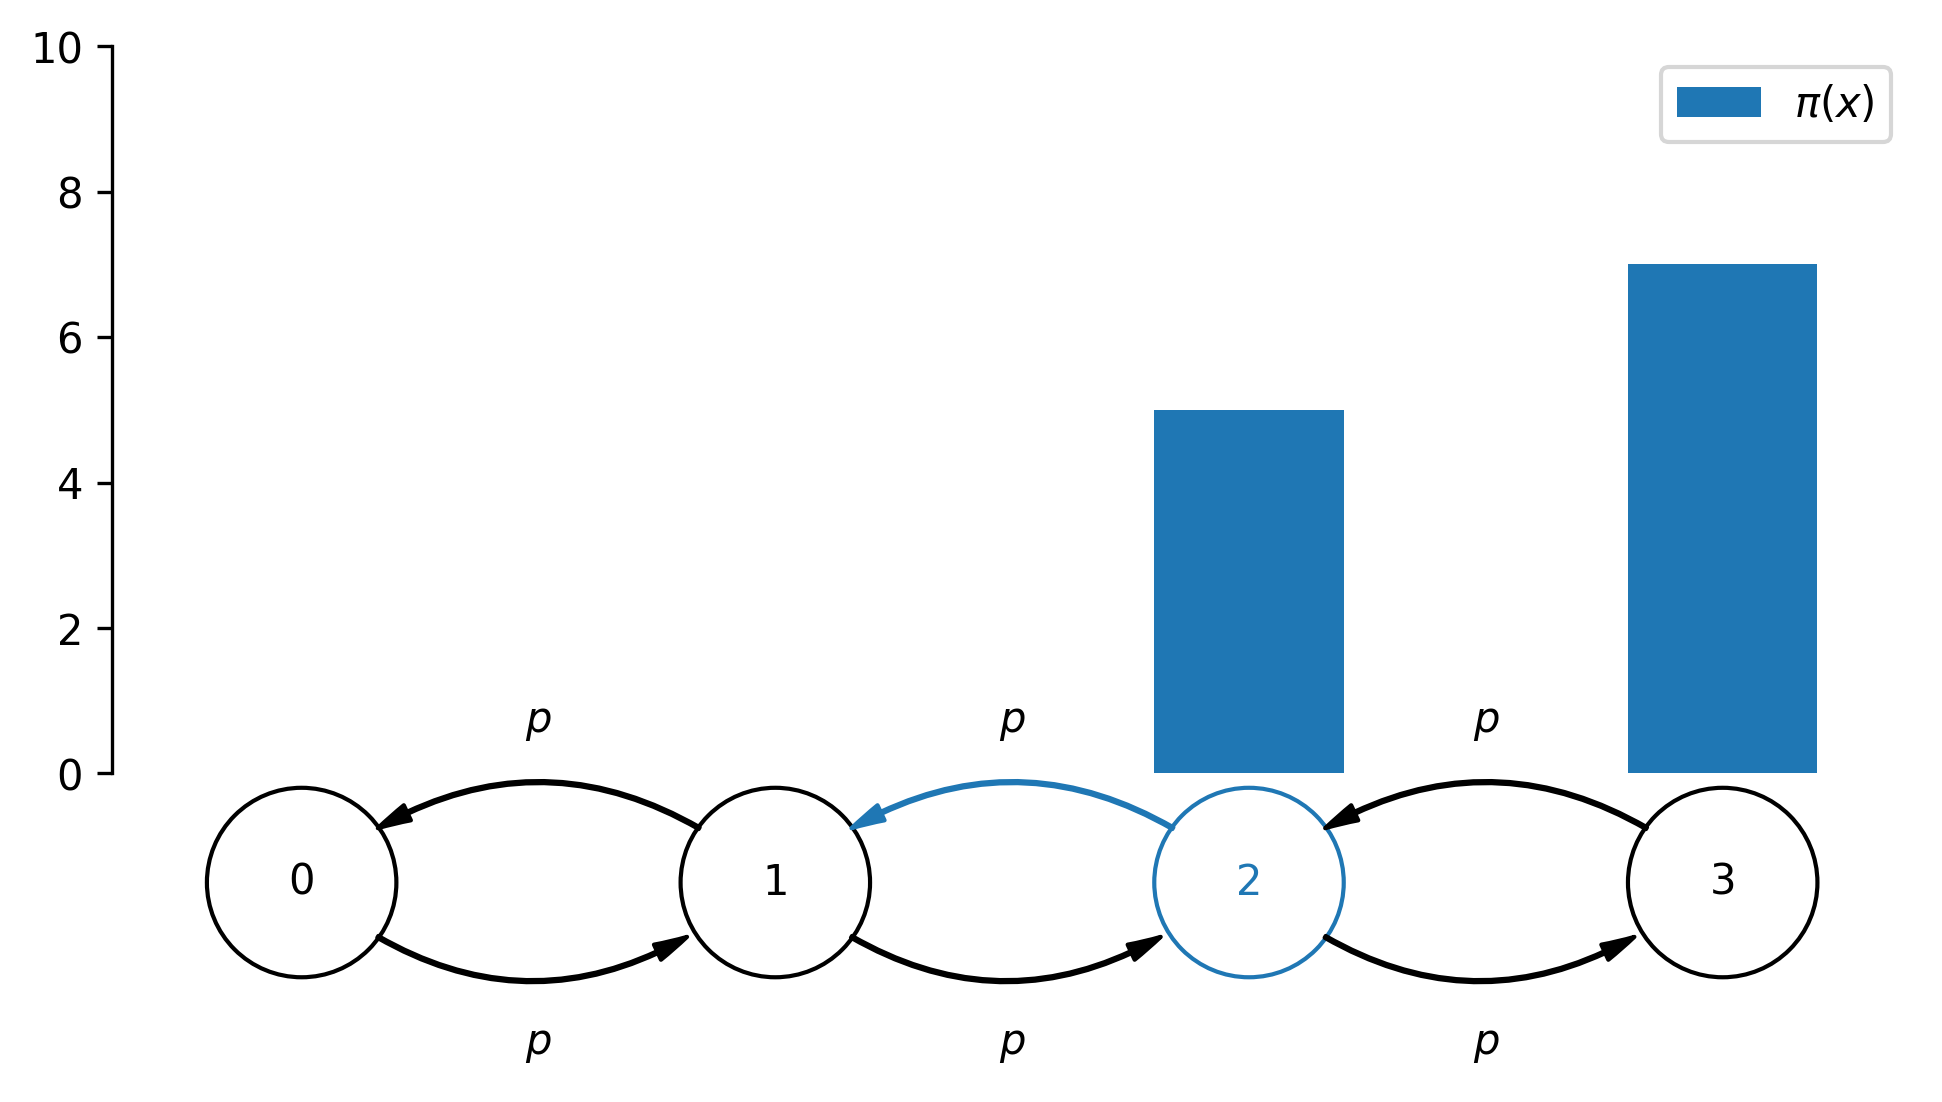
\includegraphics[scale=0.6]{imgs/simulation11.png}
    \end{center}
\end{frame}

\begin{frame}[c]
    \frametitle{Markov Chains ...}
    \begin{itemize}
        \item We simulate and count ...
    \end{itemize}
    \begin{center}
        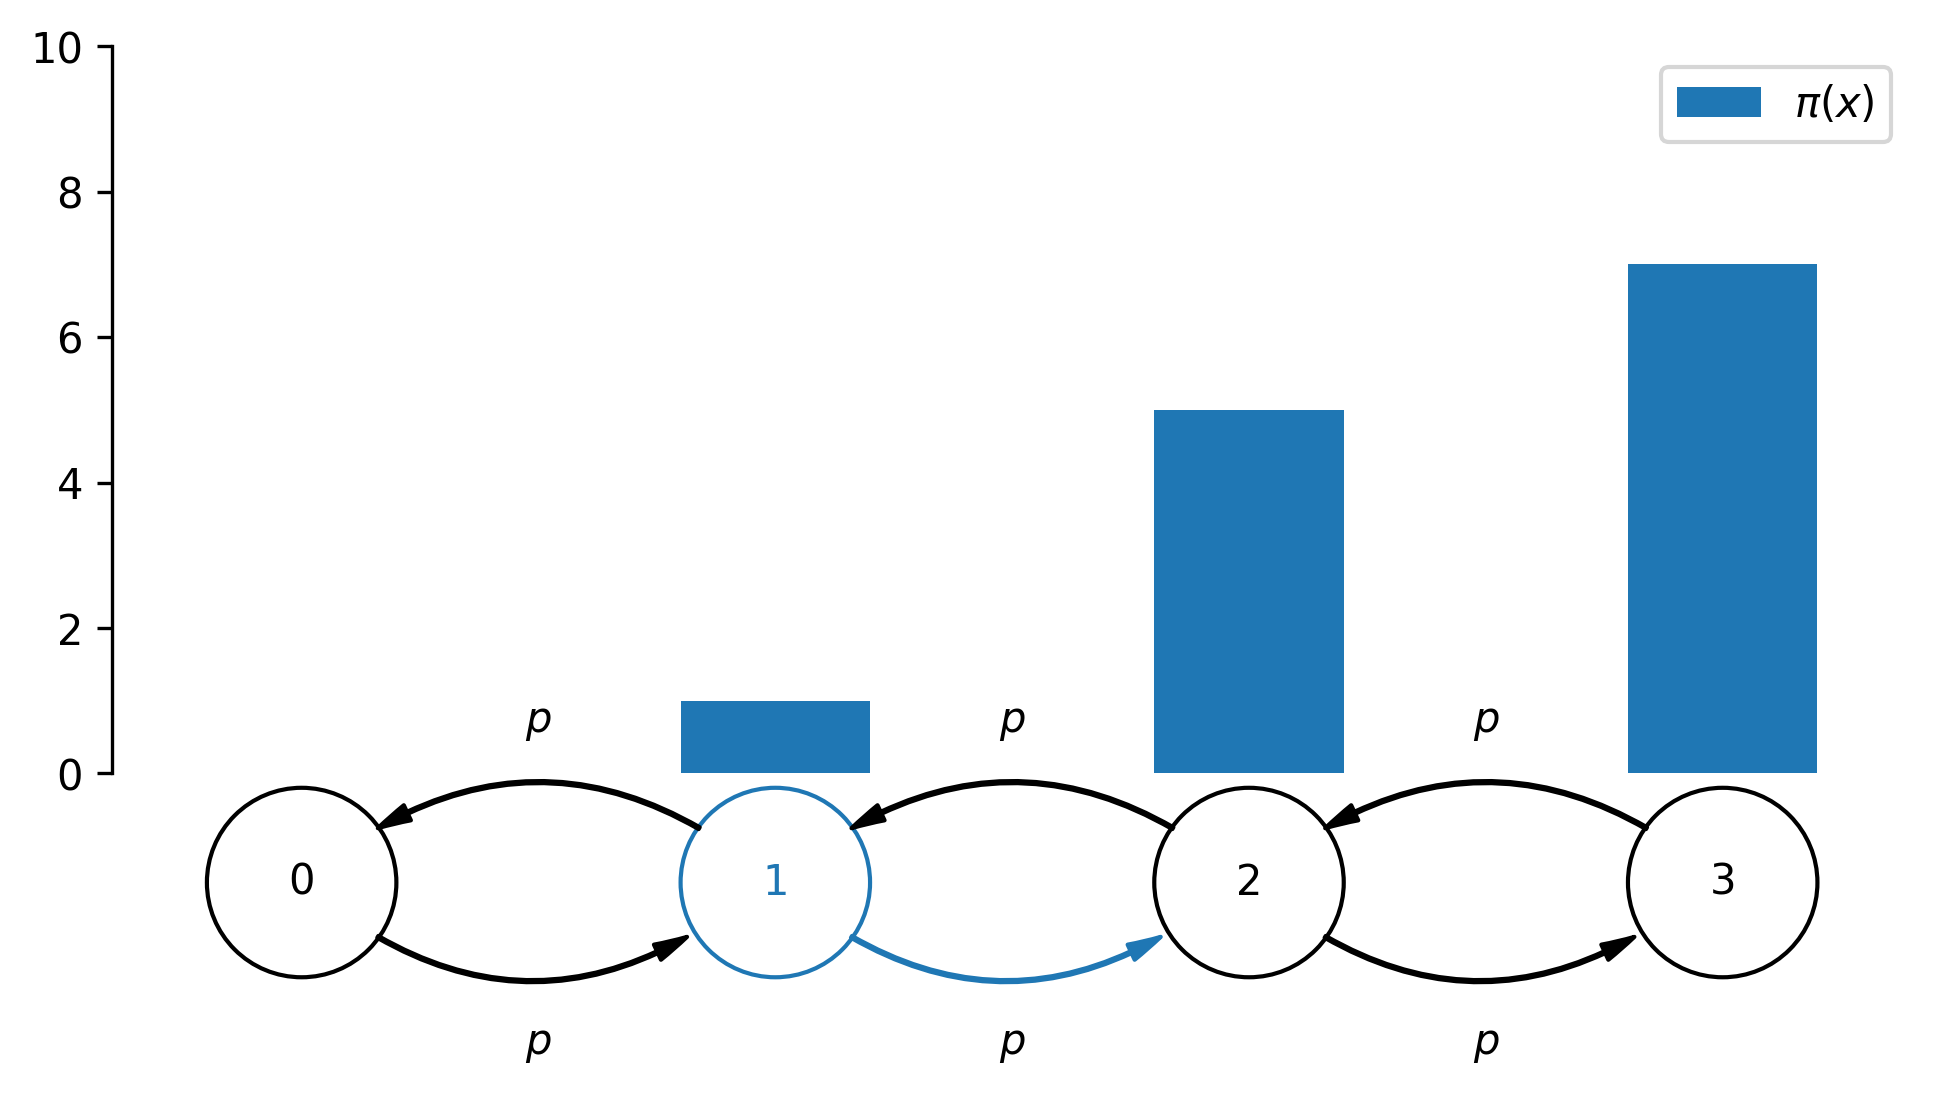
\includegraphics[scale=0.6]{imgs/simulation12.png}
    \end{center}
\end{frame}

\begin{frame}[c]
    \frametitle{Markov Chains ...}
    \begin{itemize}
        \item We simulate and count ...
    \end{itemize}
    \begin{center}
        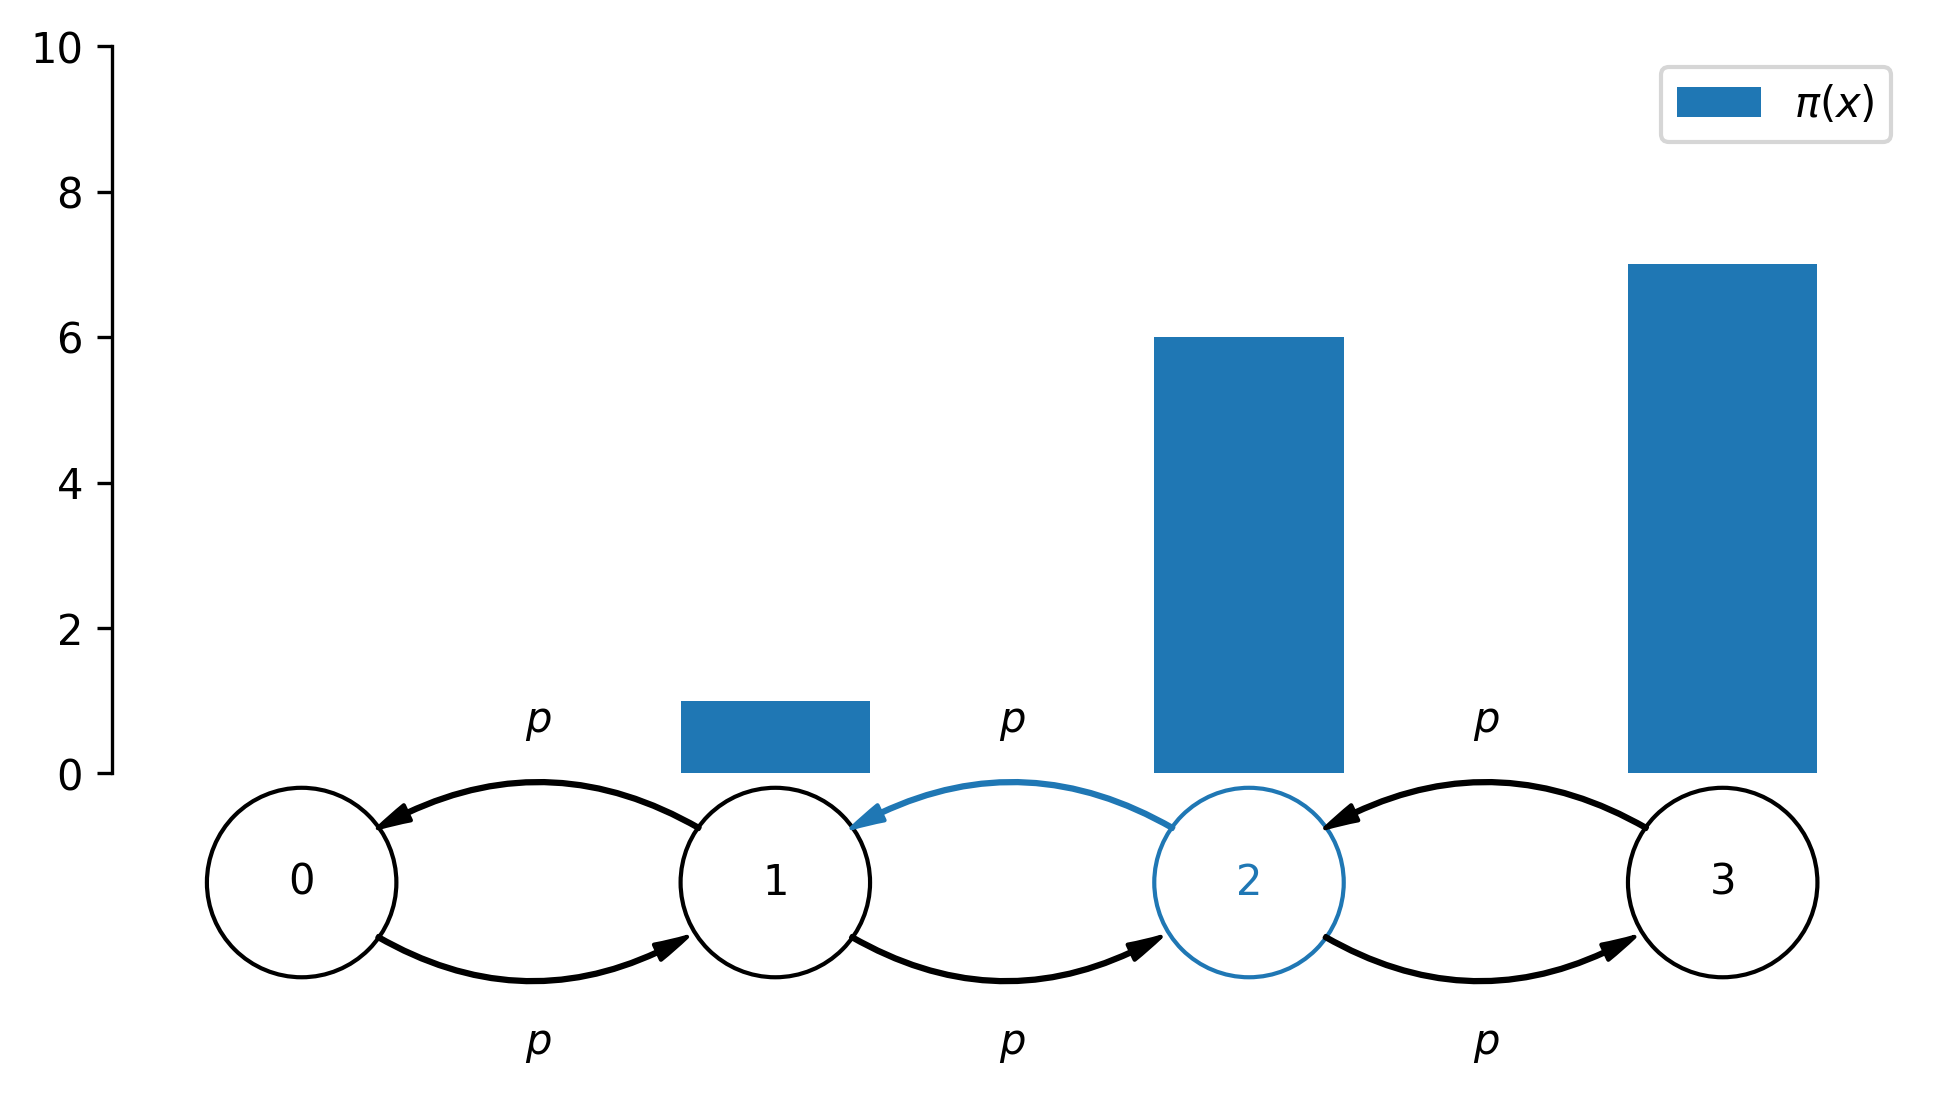
\includegraphics[scale=0.6]{imgs/simulation13.png}
    \end{center}
\end{frame}

\begin{frame}[c]
    \frametitle{Markov Chains ...}
    \begin{itemize}
        \item We simulate and count ...
    \end{itemize}
    \begin{center}
        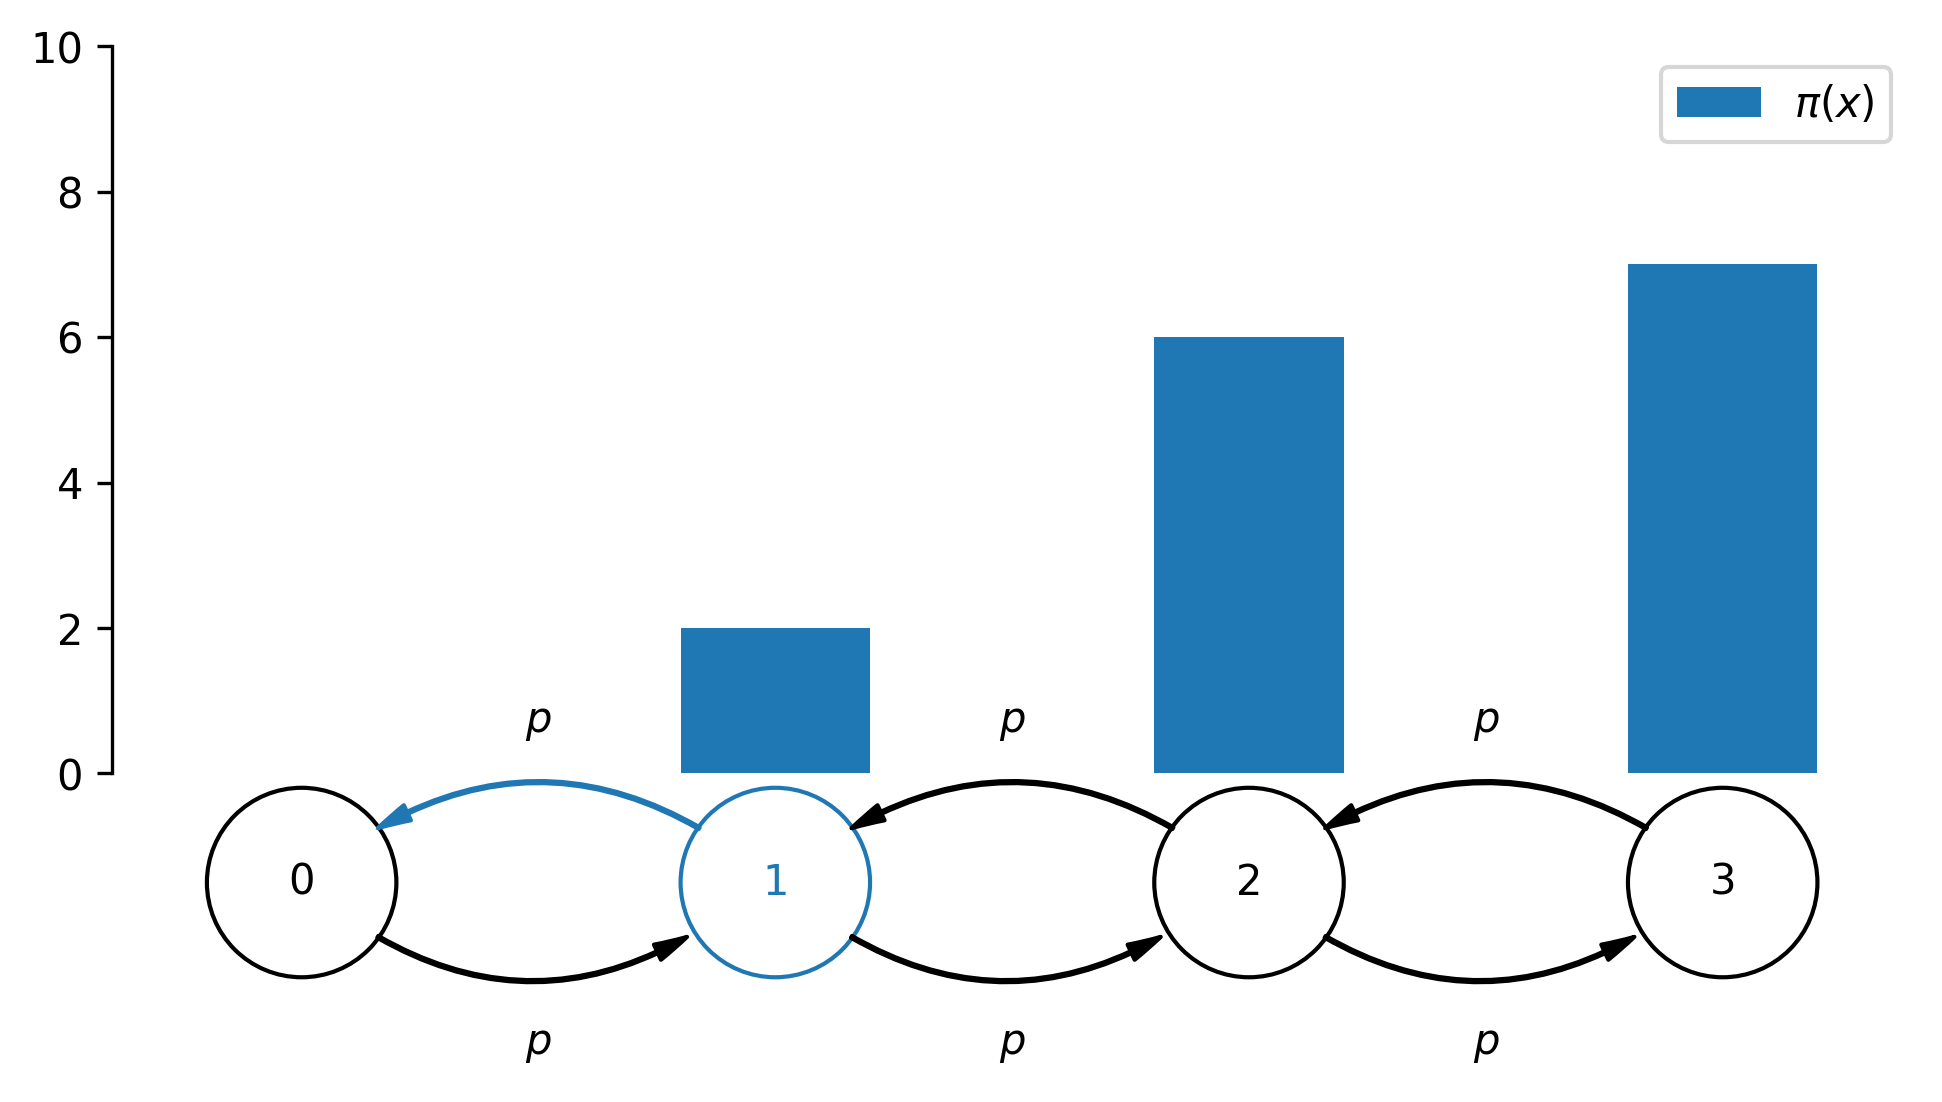
\includegraphics[scale=0.6]{imgs/simulation14.png}
    \end{center}
\end{frame}

\begin{frame}[c]
    \frametitle{Markov Chains ...}
    \begin{itemize}
        \item At some point, we would reach the \emph{invariant} or \emph{equilibrium distribution} $\pi$
            \begin{align*}
                \pi = P \pi
            \end{align*}
    \end{itemize}
    \vspace{-0.5cm}
    \begin{center}
        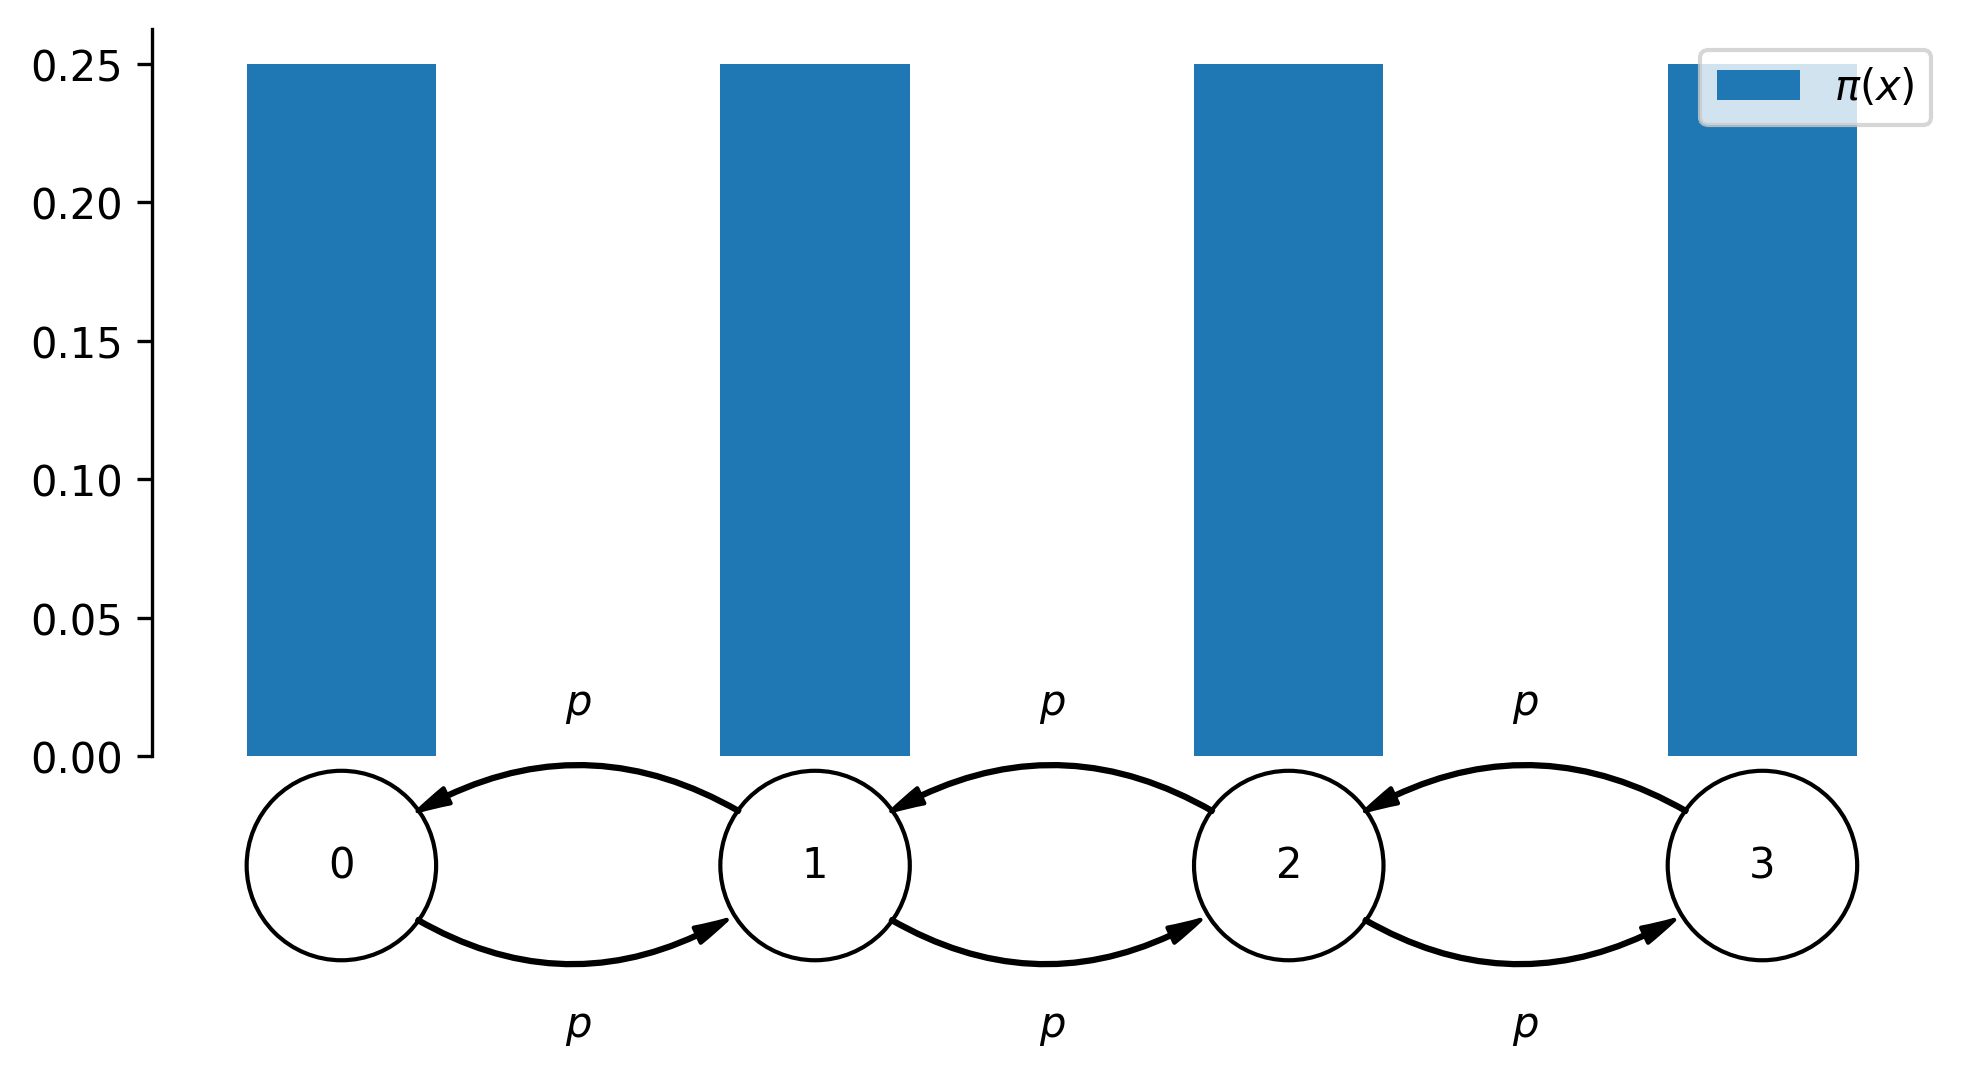
\includegraphics[scale=0.5]{imgs/uniformchaindistribution.png}
    \end{center}
    \vspace{-0.3cm}
    \begin{itemize}
        \item Theory also tells us, that under suitable conditions (e.g finite $\Theta$), we have that
            \vspace{-0.1cm}
            \begin{align*}
                \lim_{n\to \infty} (P^n)_i = \pi \quad \forall i \in \Theta
            \end{align*}
    \end{itemize}
\end{frame}

\begin{frame}[c]
    \frametitle{Markov Chains ...}
    \begin{itemize}
        \item We went from given transition matrix $P$ to the \textbf{unique} invariant distribution $\pi$
        \item We can also go from given invariant distribution $\pi$ (or measure!) to \textbf{non-unique} transition probabilities $P$!
        \item Given $\pi$, we have 
            \begin{align*}
                \pi_i &= \sum_j \pi_j P_{ji} \\
                \underbrace{\sum_j P_{ij}}_{=1} \pi_i &= \sum_j \pi_j P_{ji} 
            \end{align*}
        \item Now, 
            \begin{align*}
            \underbrace{\pi_i P_{ij} = \pi_j P_{ji}}_{\text{\emph{detailed balance condition}}} \implies \sum_j P_{ij} \pi_i = \sum_j \pi_j P_{ji} 
            \end{align*}
    \end{itemize}
\end{frame}

\begin{frame}[c]
    \frametitle{Markov Chains ...}
    \begin{itemize}
        \item First, rearrange ...
            \begin{align*}
                \pi_i P_{ij} = \pi_j P_{ji} \implies
                \frac{P_{ij}}{P_{ji}} = \frac{\pi_j}{\pi_i}
            \end{align*}
        \item ... and finally choose
            \begin{align*}
                P_{ij} = \min\Big\{1, \frac{\pi_j}{\pi_i}\Big\}
            \end{align*}
            the famous \textbf{Metropolis Filter}
    \end{itemize}
\end{frame}

\begin{frame}[c]
    \frametitle{... \& Stepsizes}
    \begin{itemize}
        \item In continuous space, we split the transition probability $P(\theta, \theta')$ 
            into proposal $q(\theta, \theta^*)$ and acceptance probability $\alpha(\theta, \theta^*)$ and use
            \begin{align*}
                \alpha(\theta, \theta^*) = \min\Big\{1, \frac{\pi(\theta^*)q(\theta^*, \theta)}{\pi(\theta)q(\theta, \theta^*)}\Big\}
            \end{align*}
        \item $q$ usually depends on some parameters, e.g. using 
            \[
                q(\theta, \theta^*) = q_{s}(\theta^* | \theta) \sim \mathcal{N}(\theta, s),
            \]
            what \emph{stepsize} $s$ should we use?
    \end{itemize}
\end{frame}

\begin{frame}[c]
    \frametitle{... \& Stepsizes}
    \begin{itemize}
        \item What $s$ should we use?
    \end{itemize}
    \vspace{-.8cm}
    \begin{center}
        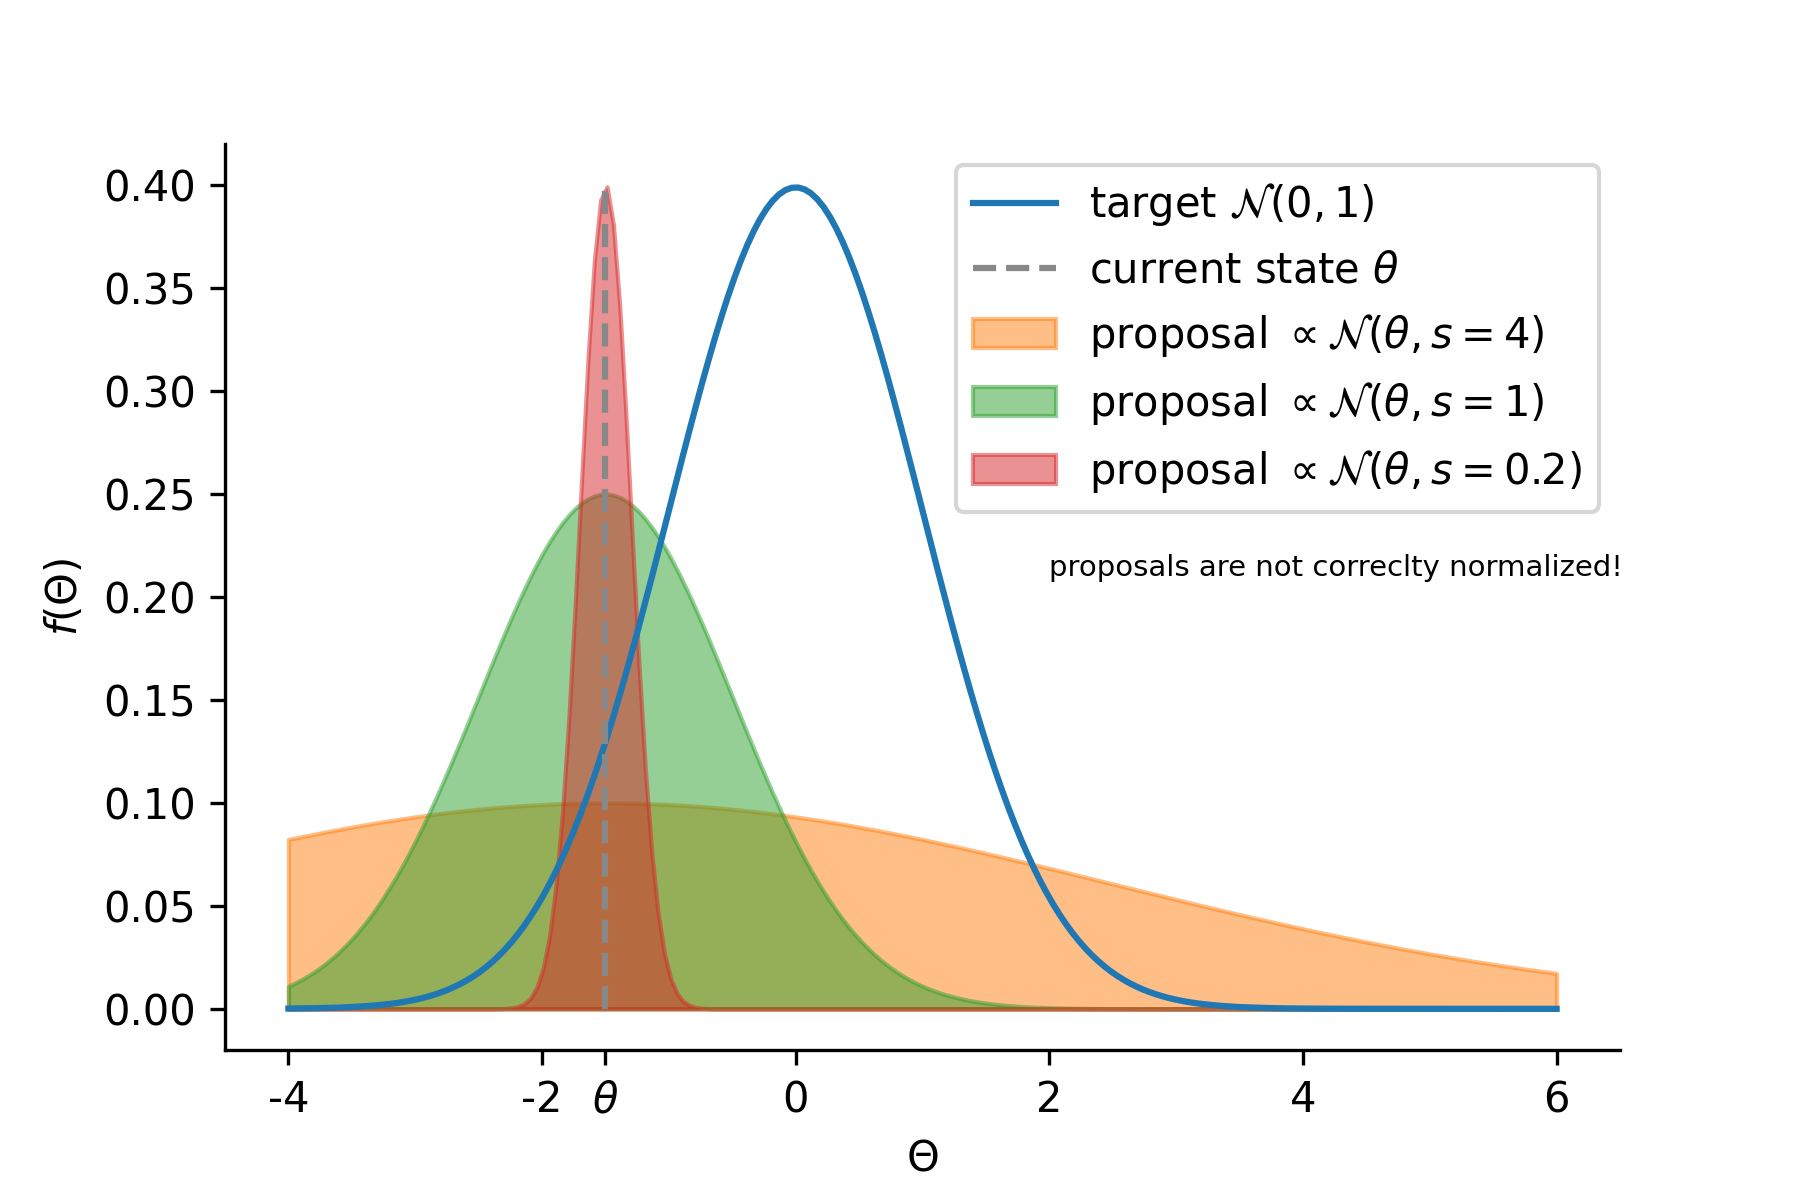
\includegraphics[scale=0.6]{imgs/stepsizes.png}
    \end{center}
    \vspace{-.5cm}
    \begin{itemize}
        \item Again: Transition kernels to a given invariant distribution are \textbf{not unique}
    \end{itemize}
\end{frame}

\begin{frame}[c]
    \frametitle{Agenda}
    \begin{itemize}
        \item Overview
        \begin{itemize}
            {\color{lgray}
            \item Markov Chains \& Stepsizes
            }
            \item Effectiveness \& Expected Squared Jump Distance 
            {\color{lgray}
            \item Thompson Sampling
            \item Once more: Why not to tune the acceptance rate!
            }
        \end{itemize}
        {\color{lgray}
        \item Results
        \item Improvements \& More
        }
        \begin{itemize}
            {\color{lgray}
            \item Acceptance Rate Tuning with Thompson Sampling
            \item Tune higher-order Autocorrelation Lags
            \item Gaussian Process Time Costs
            \item Monotonicity of Thinning
        }
        \end{itemize}
    \end{itemize}
\end{frame}

\begin{frame}[c]
    \frametitle{Effectiveness ...}
    \begin{itemize}
        \item Given samples $\theta_0, \ldots, \theta_n$,  
            the sample average is $\bar{\theta} = \frac{1}{n} \sum_{i=0}^n \theta_i$ 
            and the squared statistical error in $\bar{x}$ is the variance 
            \begin{align*}
                \mathrm{Var}[\bar{\theta}] 
                &= \mathbb{E}[\bar{\theta}^2] - \mathbb{E}[\bar{\theta}]^2 \\
                &= \frac{\sigma^2}{n^2} \bigg(n + \sum_{t = 1}^{n-1} (n-t) \rho_t\bigg) 
                    \quad \text{ with } \quad \rho_t = 
                    \frac{\mathbb{E}[\theta_0 \theta_t] - \mu^2}{\sigma^2} \\
                &= \frac{\sigma^2}{n} \bigg(1 + \sum_{t = 1}^{n-1} \Big(1-\frac{t}{n}\Big) \rho_t\bigg)
                    < \frac{\sigma^2}{n} \underbrace{\bigg(1 + \sum_{t = 1}^{n-1} \rho_t\bigg)}_{=:\tau}
            \end{align*}
        \item From this we derive the effective sample size as
            \[
                \mathrm{Var}[\bar{x}] = \frac{\sigma^2}{n_{\mathrm{eff}}} \quad \text{ with } \quad n_\mathrm{eff} = \frac{n}{\tau}
            \]
    \end{itemize}
\end{frame}

\begin{frame}[c]
    \frametitle{Effectiveness ...}
    \begin{itemize}
        \item The effective sample size is commonly used as a measure of quality for Markov chains
        \begin{itemize}
            \item Note that $\tau = \tau\big((\theta_t)_{t=0}^n\big)$ and $(\theta_t)_{t=0}^n = \big((\theta_t)_{t=0}^n\big)(s)$
        \end{itemize}
        \item We now increase effectiveness by reducing $\tau$, since $n_\mathrm{eff} = \frac{n}{\tau}$
        \item Autocorrelations are usually assumed to be decreasing in time: $\rho_t \geq \rho_{t+k},$ for $k \geq 1$
        \item Thus, \textbf{decrease autocorrelation for small lags}!
    \end{itemize}
\end{frame}

\begin{frame}[c]
    \frametitle{... \& Expected Squared Jump Distance}
    \begin{itemize}
        \item We define
        \begin{align*}
            \mathrm{ESJD(\theta)} := \mathbb{E}[(\theta_{t+1} - \theta_t)^2] 
                &= \underbrace{\mathbb{E}[\theta_{t+1}^2]}_{=\mathbb{E}[\theta^2]} - 2\mathbb{E}[\theta_{t+1}\theta_t] + \underbrace{\mathbb{E}[\theta_t^2]}_{=\mathbb{E}[\theta^2]} \\
                &= 2\big(\mathbb{E}[\theta^2] - \mathbb{E}[\theta_{t+1}\theta_t]  + \mu^2 - \mu^2\big)\\
                &= 2\big(\sigma^2 - \big(\mathbb{E}[\theta_{t+1}\theta_t]  - \mu^2\big)\big)\\
                &= 2\sigma^2\big(1 - \frac{\mathbb{E}[\theta_{t+1}\theta_t]  - \mu^2}{\sigma^2}\big)\\
                &= 2\sigma^2\big(1 - \rho_1\big)
        \end{align*}
        \item Since $\sigma^2$ is constant, maximizing the ESJD reduces the lag-1 autocorrelation, \textbf{increasing efficiency}.
    \end{itemize}
\end{frame}

\begin{frame}[c]
    \frametitle{... \& Expected Squared Jump Distance}
    \begin{itemize}
        \item However, the ESJD is a function of the \textbf{unknown} true target distribution, so we have to \textbf{estimate} it.
        \item We have a guess, how the function $\mathrm{ESJD}(s)$ looks like, but in general, it remains a black box function.
        \item[] $\implies$ \textbf{Thompson Sampling}
    \end{itemize}
\end{frame}

\begin{frame}[c]
    \frametitle{Agenda}
    \begin{itemize}
        \item Overwiew
        \begin{itemize}
            {\color{lgray}
            \item Markov Chains \& Stepsizes
            \item Effectiveness \& Expected Squared Jump Distance 
            }
            \item Thompson Sampling
            {\color{lgray}
            \item Once more: Why not to tune the acceptance rate!
            }
        \end{itemize}
        {\color{lgray}
        \item Results
        \item Improvements \& More
        }
        \begin{itemize}
            {\color{lgray}
            \item Acceptance Rate Tuning with Thompson Sampling
            \item Tune higher-order Autocorrelation Lags
            \item Gaussian Process Time Costs
            \item Monotonicity of Thinning
        }
        \end{itemize}
    \end{itemize}
\end{frame}

\begin{frame}[c]
    \frametitle{Thompson Sampling}
    \begin{itemize}
        \item A Bayesian optimization approach to optimize an unknown \textbf{black box} objective function:
        \begin{itemize}
            \item We can evaluate it pointwise, but that's it!
        \end{itemize}
        \item Thus, we have to explore the function and search for the optimum simultaneously
        \item[]
        \item Thompson Sampling:
        \begin{itemize}
            \item Assume a distribution over the possible shapes of the black box function
            \item Sample that distribution and evaluate the black box function, where the sampled function is maximized
            \item Update the distribution over the possible function shapes based on the observed evaluation
        \end{itemize}
    \end{itemize}
\end{frame}

\begin{frame}[c]
    \frametitle{Going to the restaurant!}
    \begin{itemize}
        \item You're coming to Vienna and there exist a total of 5 different restaurants, the internet has not yet been invented, I never went out in 8 years here
        \item Any restaurant might be good or bad, so we choose the first one uniformly
        \item[] $\implies$ We already assumed a (uniform) distribution over the restaurants quality!
    \end{itemize}
    \vspace{-.5cm}
    \begin{center}
        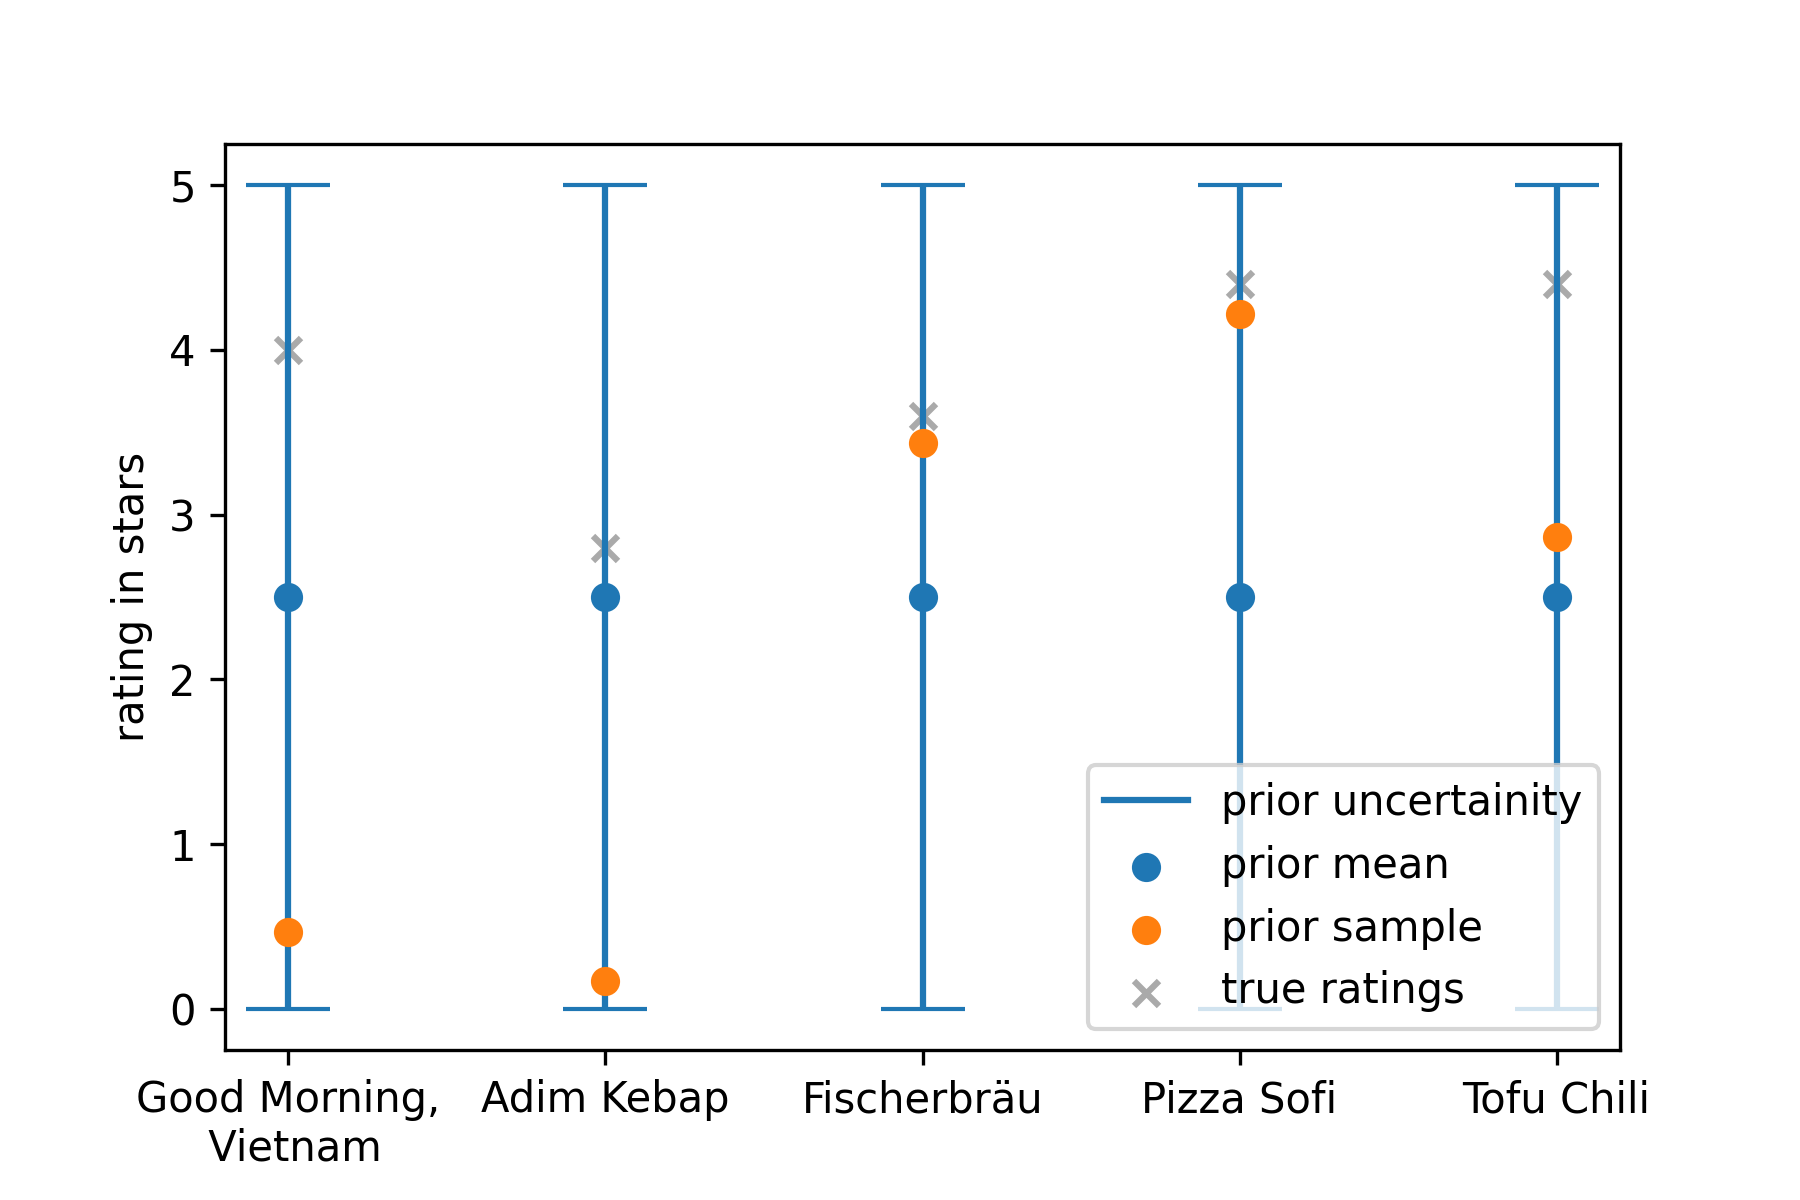
\includegraphics[scale=0.5]{imgs/restaurantsprior.png}
    \end{center}
\end{frame}

\begin{frame}[c]
    \frametitle{Going to the restaurant!}
    \begin{itemize}
        \item We go to \emph{Pizza Sofi} and rate it with 4 stars, but we only had a fraction of their menu
        \item Would we have rated the same, if we had eaten something else? Did the cook have an exceptional good day?
        \item[] $\implies$ There is function noise and uncertainity left in our rating!
    \end{itemize}
    \vspace{-.5cm}
    \begin{center}
        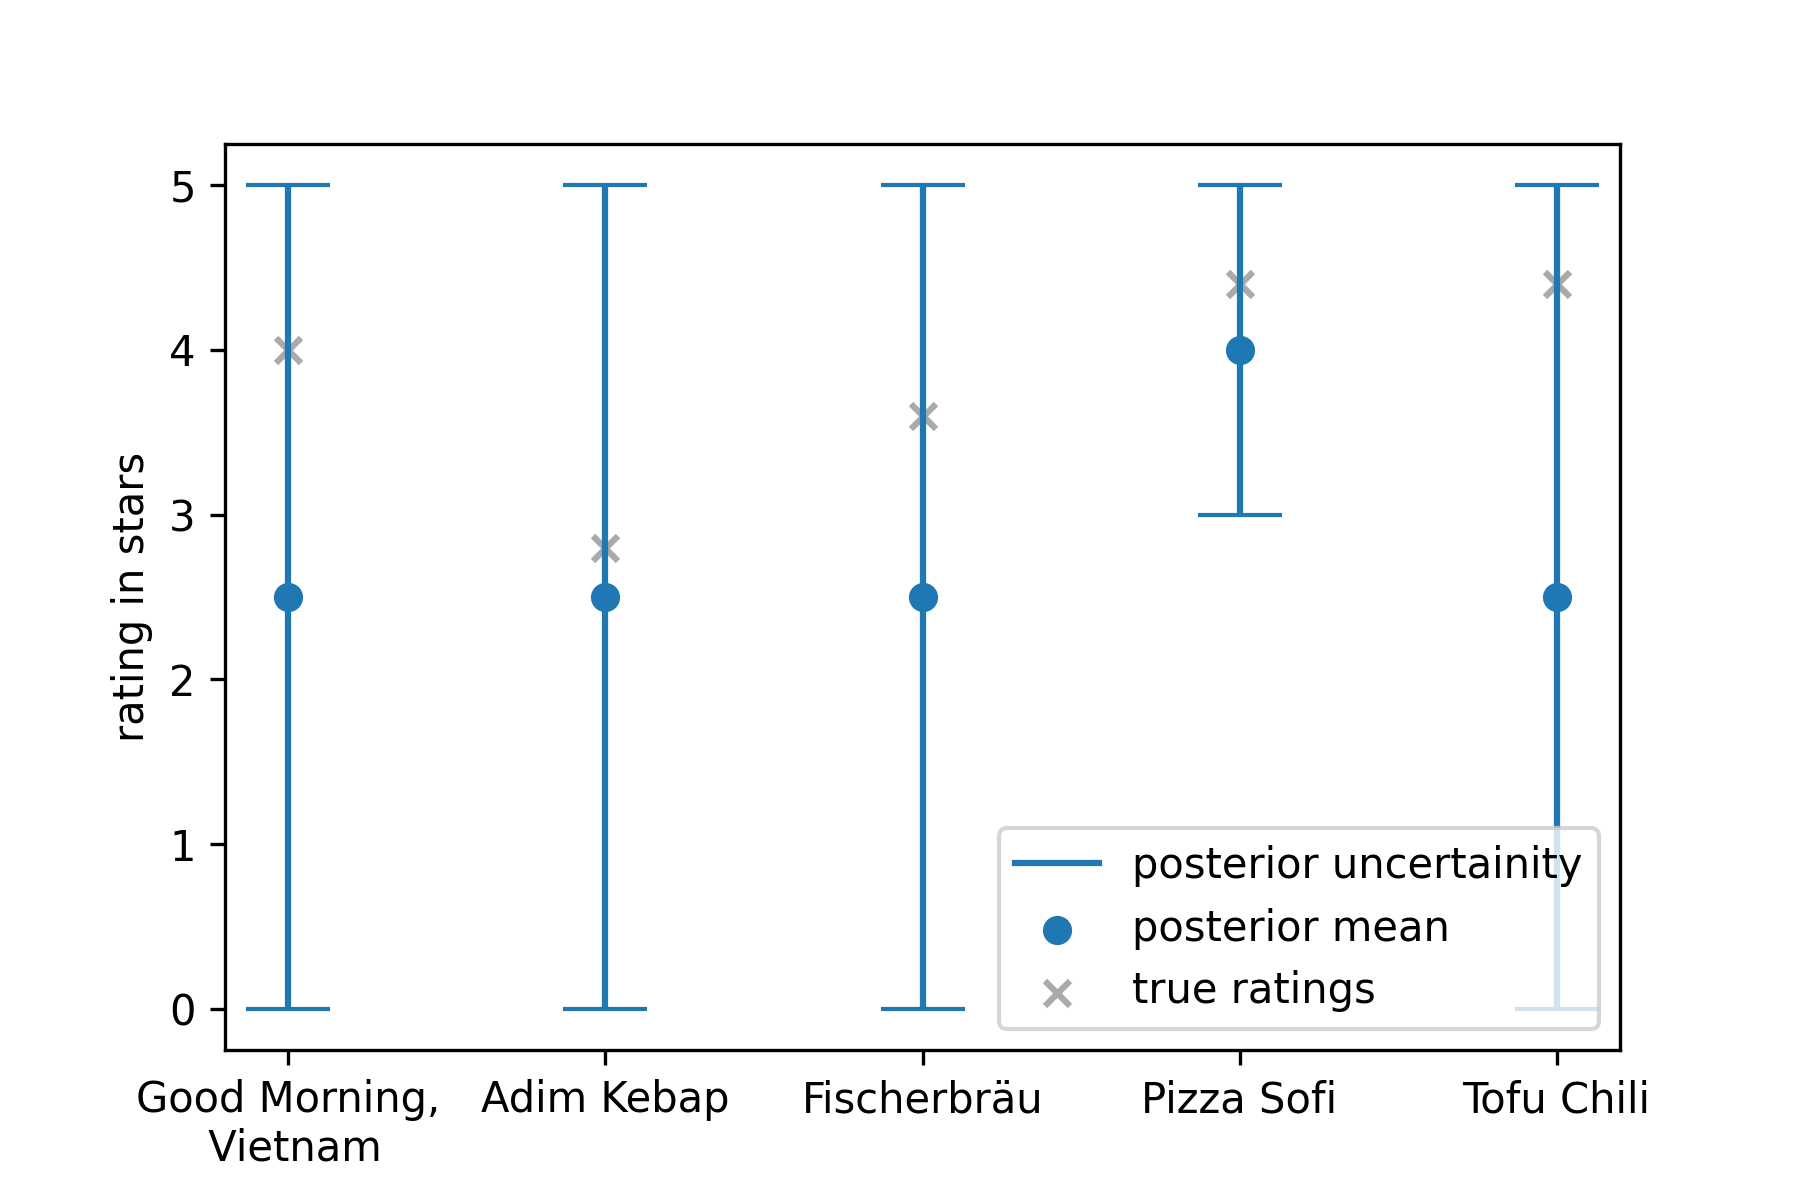
\includegraphics[scale=0.5]{imgs/restaurantsposterior.png}
    \end{center}
\end{frame}

\begin{frame}[c]
    \frametitle{Going to the restaurant!}
    \begin{itemize}
        \item Once more, we want to go out eating. What restaurant to choose? 
        \item "Sample" from your posterior belief about the quality of the restaurants and go to the one, 
            where your sample tells you, that you will have the best experience:
        \item Afterwards, update your beliefs based on your experience.
    \end{itemize}
    \vspace{-.5cm}
    \begin{center}
        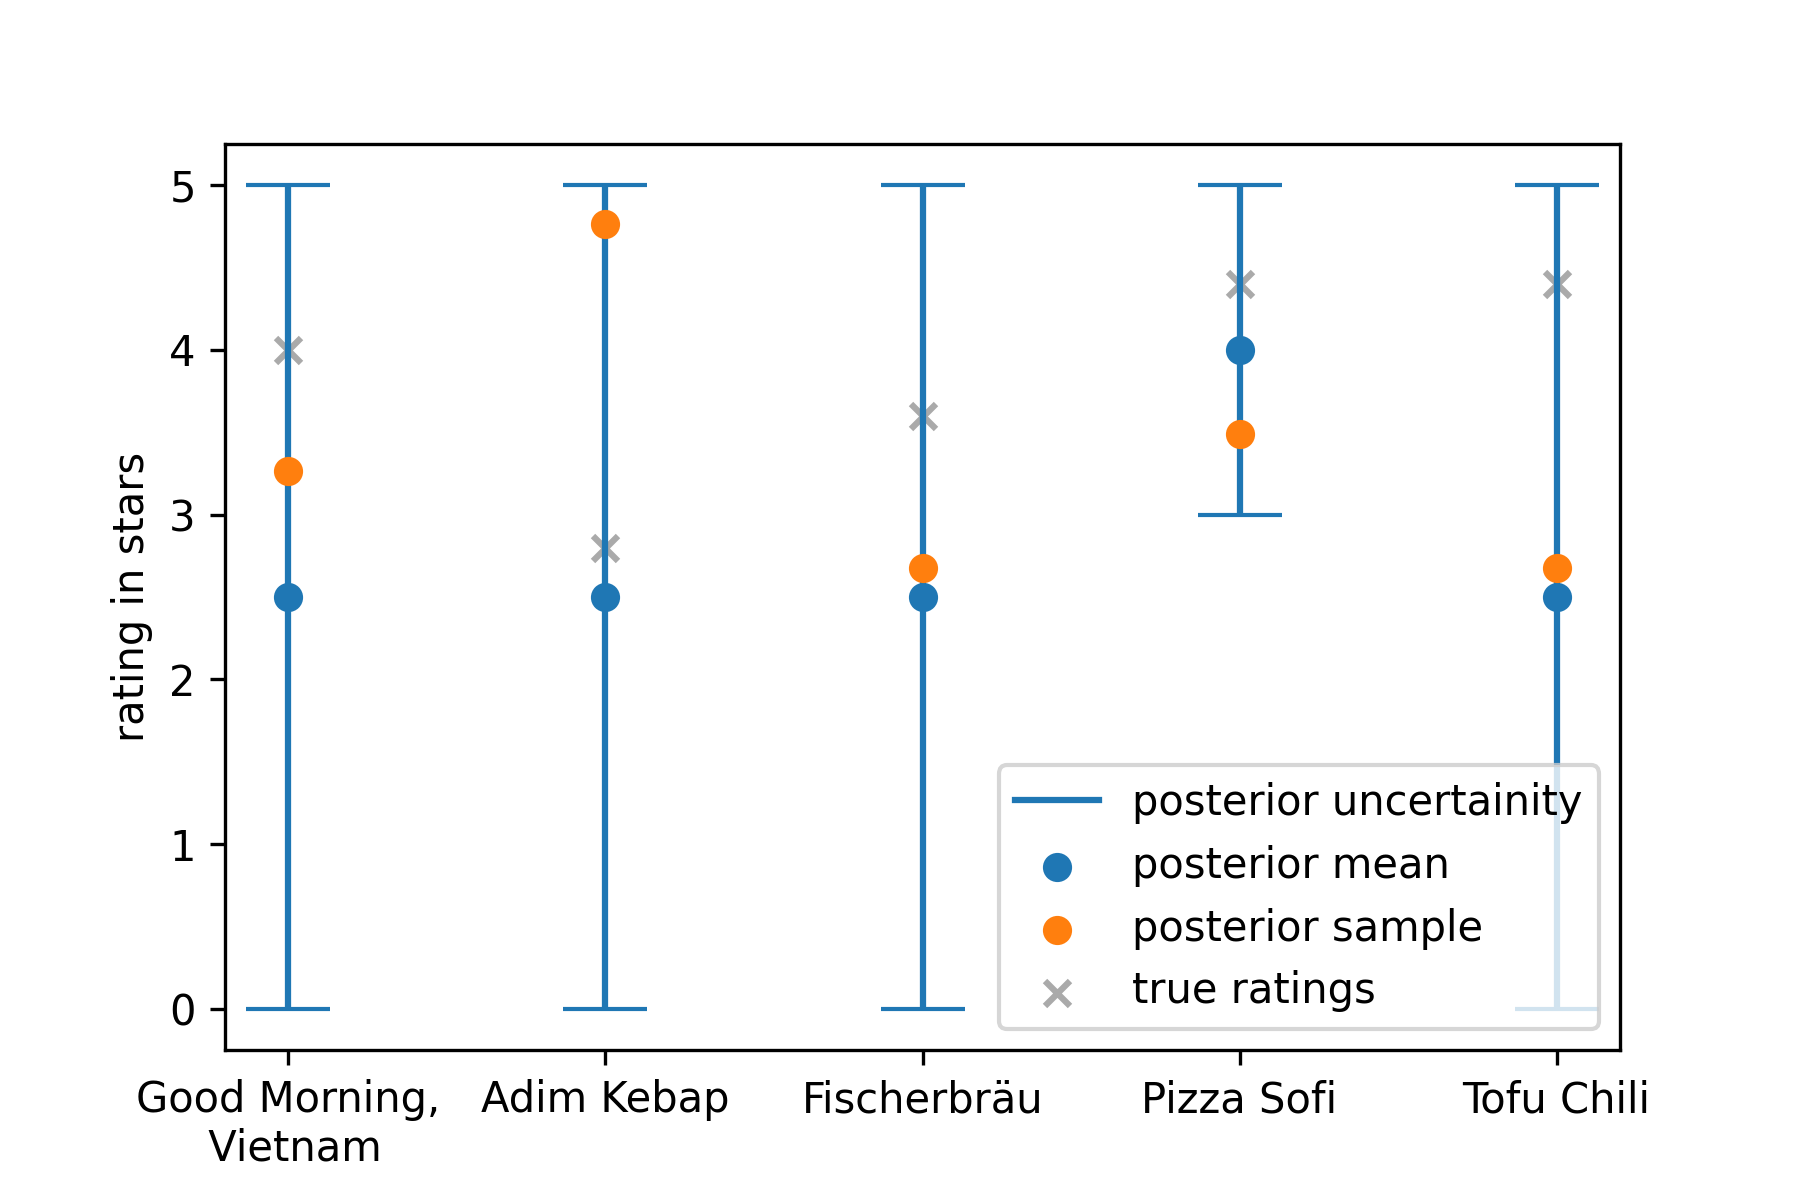
\includegraphics[scale=0.5]{imgs/restaurantsposteriorwsample.png}
    \end{center}
\end{frame}

\begin{frame}[c]
    \frametitle{Dinner with William Thompson and Andrey Markov}
    \begin{itemize}
        \item Our restaurants are the stepsizes $s$, that we test.
        \item[]
        \item Our friends, with whom we go to the restaurant, is the number of chains, that we use.
        \item[] $\implies$ Each friend rates the restaurant differently, each chain measures another value \\
            \phantom{$\implies$} for the objective function
        \item[]
        \item The amount of money we spend, is the number of samples, we use to test the stepsize
        \item[] $\implies$ We never take everything, that the restaurant has to offer. But taking more \\
            \phantom{$\implies$} than just a salad is likely to reveal more about the kitchen's qualities, that is \\
            \phantom{$\implies$} reduce the error in the estimate of the objective function
    \end{itemize}
\end{frame}

\begin{frame}[c]
    \frametitle{More formal Thompson Sampling}
    \begin{itemize}
        \item We model our distribution over the possible black box functions as a Gaussian Process (GP)
        \item The algorithm then is:
            \begin{algorithm2e}[H]
                \For{$t \in 0, \ldots, m$}{
                    sample $\hat{f}_t \sim GP(\mu_t, \Sigma_t)$ \\
                    let $x_t := \mathrm{arg\,max} \, \hat{f}_t(x)$ \\
                    let $y_t := f(x_t)$ \\
                    let $D_{t+1} := D_t \cup \{(x_t, y_t)\}$ \\
                    update $\mu_{t+1}$ using $D_{t+1}$ \\
                    update $\Sigma_{t+1}$ using $D_{t+1}$ \\
                }
            \end{algorithm2e}
    \end{itemize}
\end{frame}

\begin{frame}[c]
    \frametitle{Agenda}
    \begin{itemize}
        \item Overwiew
        \begin{itemize}
            {\color{lgray}
            \item Markov Chains \& Stepsizes
            \item Effectiveness \& Expected Squared Jump Distance 
            \item Thompson Sampling
            }
            \item Once more: Why not to tune the acceptance rate!
        \end{itemize}
        {\color{lgray}
        \item Results
        \item Improvements \& More
        }
        \begin{itemize}
            {\color{lgray}
            \item Acceptance Rate Tuning with Thompson Sampling
            \item Tune higher-order Autocorrelation Lags
            \item Gaussian Process Time Costs
            \item Monotonicity of Thinning
        }
        \end{itemize}
    \end{itemize}
\end{frame}

\begin{frame}[c]
    \frametitle{Once more: Why not to tune the acceptance rate!}
    \begin{itemize}
        \item 
    \end{itemize}
\end{frame}

\begin{frame}[c]
    \frametitle{Agenda}
    \begin{itemize}
        {\color{lgray}
        \item Overwiew
        }
        \begin{itemize}
            {\color{lgray}
            \item Markov Chains \& Stepsizes
            \item Effectiveness \& Expected Squared Jump Distance 
            \item Thompson Sampling
            \item Once more: Why not to tune the acceptance rate!
            }
        \end{itemize}
        \item Results
        {\color{lgray}
        \item Improvements \& More
        }
        \begin{itemize}
            {\color{lgray}
            \item Acceptance Rate Tuning with Thompson Sampling
            \item Tune higher-order Autocorrelation Lags
            \item Gaussian Process Time Costs
            \item Monotonicity of Thinning
        }
        \end{itemize}
    \end{itemize}
\end{frame}

\begin{frame}[c]
    \frametitle{Results}
    \begin{itemize}
        \item 
    \end{itemize}
\end{frame}

\begin{frame}[c]
    \frametitle{Agenda}
    \begin{itemize}
        {\color{lgray}
        \item Overwiew
        }
        \begin{itemize}
            {\color{lgray}
            \item Markov Chains \& Stepsizes
            \item Effectiveness \& Expected Squared Jump Distance 
            \item Thompson Sampling
            \item Once more: Why not to tune the acceptance rate!
            }
        \end{itemize}
        {\color{lgray}
        \item Results
        }
        \item Improvements \& More
        \begin{itemize}
            \item Acceptance Rate Tuning with Thompson Sampling
            {\color{lgray}
            \item Tune higher-order Autocorrelation Lags
            \item Gaussian Process Time Costs
            \item Monotonicity of Thinning
        }
        \end{itemize}
    \end{itemize}
\end{frame}

\begin{frame}[c]
    \frametitle{Acceptance Rate Tuning with Thompson Sampling}
    \begin{itemize}
        \item Formally, the acceptance rate is
            \begin{align*}
                \alpha = \int_{\Theta^2} \underbrace{\pi(\theta)}_{!!} q(\theta, \theta^*) \alpha(\theta, \theta^*) \, \dd \theta \, \dd \theta^*
            \end{align*}
            and thus it is a function of the \textbf{unknown} true target distribution
        \item Once more, we can only \textbf{estimate} it:
            \begin{align*}
                \hat{\alpha}(s) = \frac{1}{n}\sum_{i=0}^n \mathbbm{1}_{\{\theta_{t+1} \neq \theta_t\}} = \frac{\text{\#accepted moves}}{n}
            \end{align*}
        \item As a function of the stepsize the acceptance rate is \textbf{strictly monotonous}
        \item Use \textbf{binary search} to find the intersection of $\alpha(s)$ with some desired target value $\alpha^*$?
    \end{itemize}
\end{frame}

\begin{frame}[c]
    \frametitle{Acceptance Rate Tuning with Thompson Sampling}
    \begin{itemize}
        \item Use \textbf{binary search} to find the intersection of $\alpha(s)$ with some desired target value $\alpha^*$?
    \end{itemize}
    \vspace{-0.8cm}
    \begin{center}
        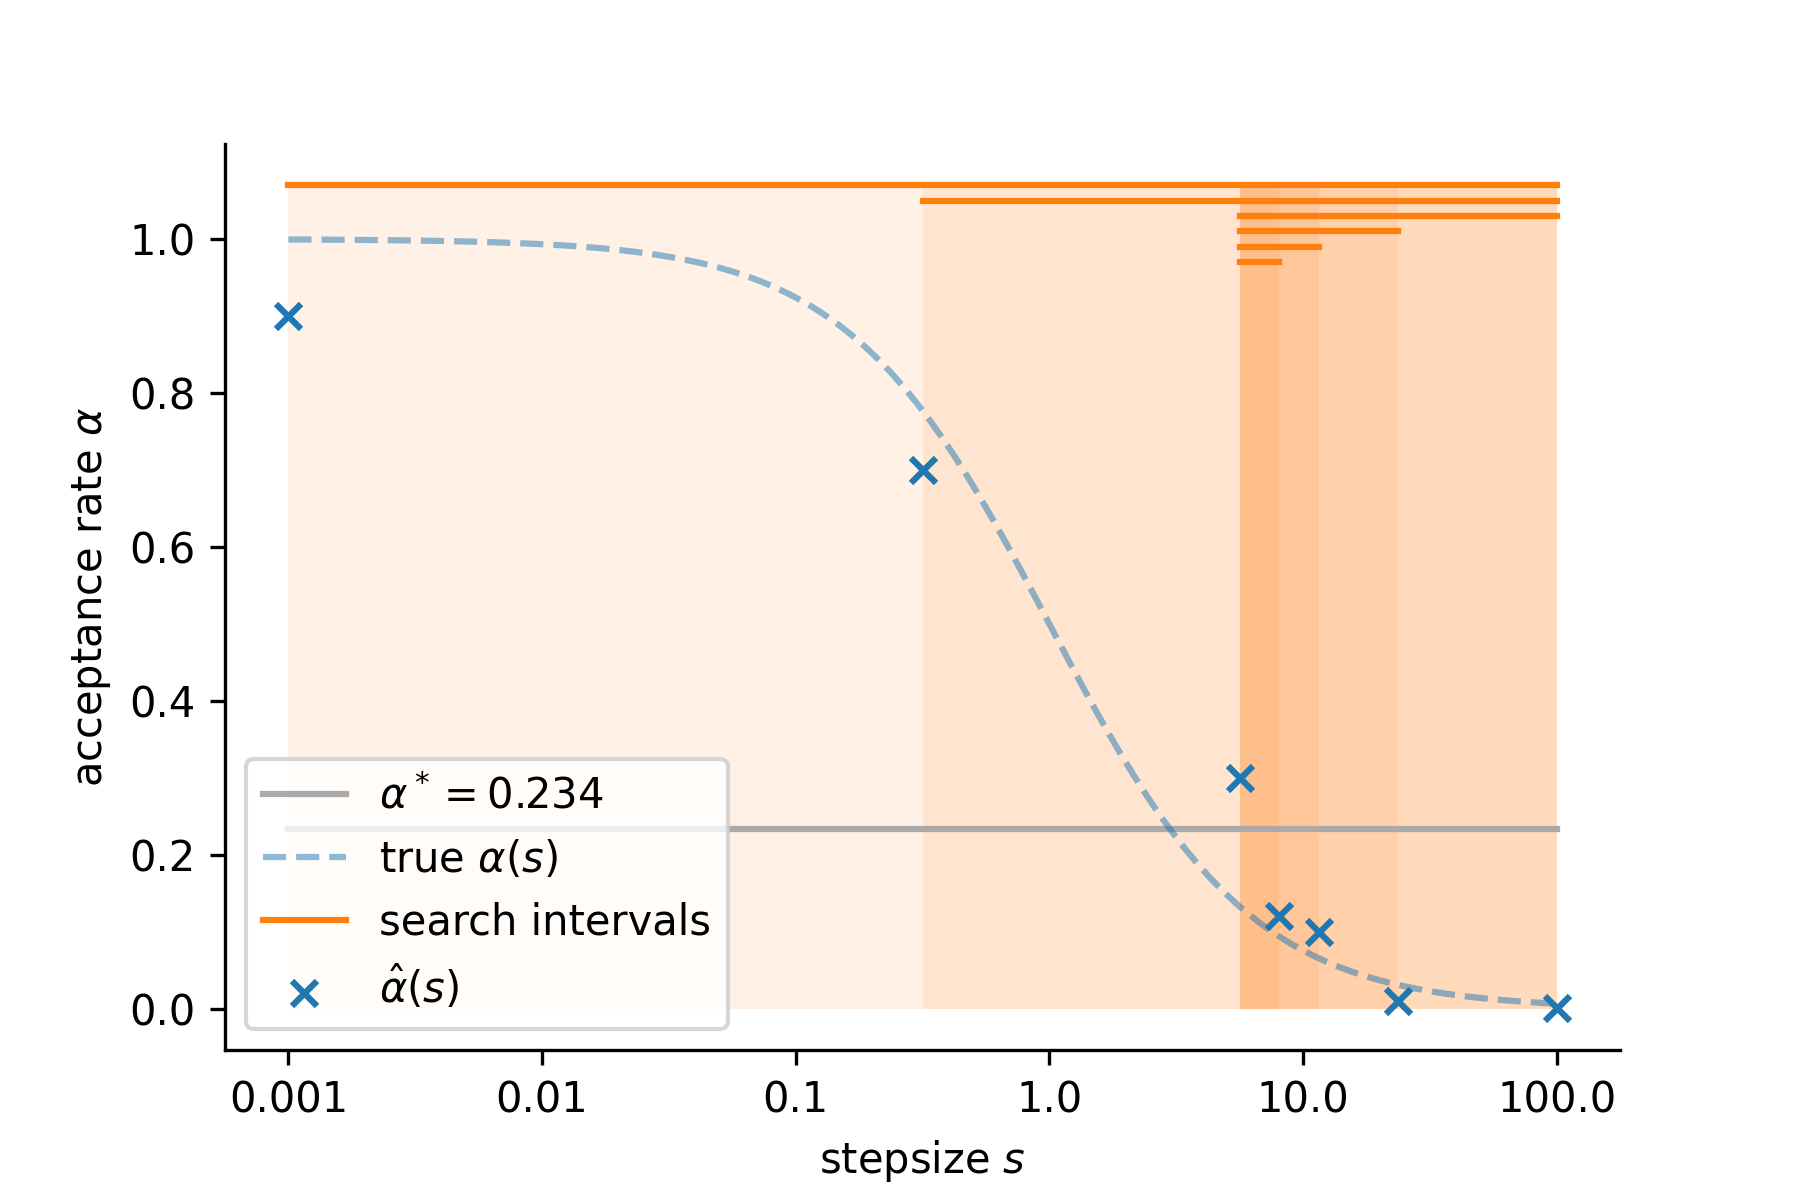
\includegraphics[scale=0.5]{imgs/nestedintervalsfailure.png}
    \end{center}
    \vspace{-0.5cm}
    \begin{itemize}
        \item \textbf{No!} This fails with noisy function evaluations which the estimator $\hat{\alpha}(s)$ gives us!
        \item[] $\to$ \emph{too deterministic!} Instead, use Thompson Sampling!
    \end{itemize}
\end{frame}

\begin{frame}[c]
    \frametitle{Acceptance Rate Tuning with Thompson Sampling}
    \begin{itemize}
        \item Given $\alpha^*$ and $\hat{\alpha}(s)$, define the score function:
            \begin{align*}
                h(s) := 1 - \Delta_\alpha := 1 - | \alpha^* - \hat{\alpha}(s)|
            \end{align*}
            which is maximized when $\hat{\alpha}(s) = \alpha^*$ and takes values in $[0,1]$
    \end{itemize}
    \vspace{-0.8cm}
    \begin{center}
        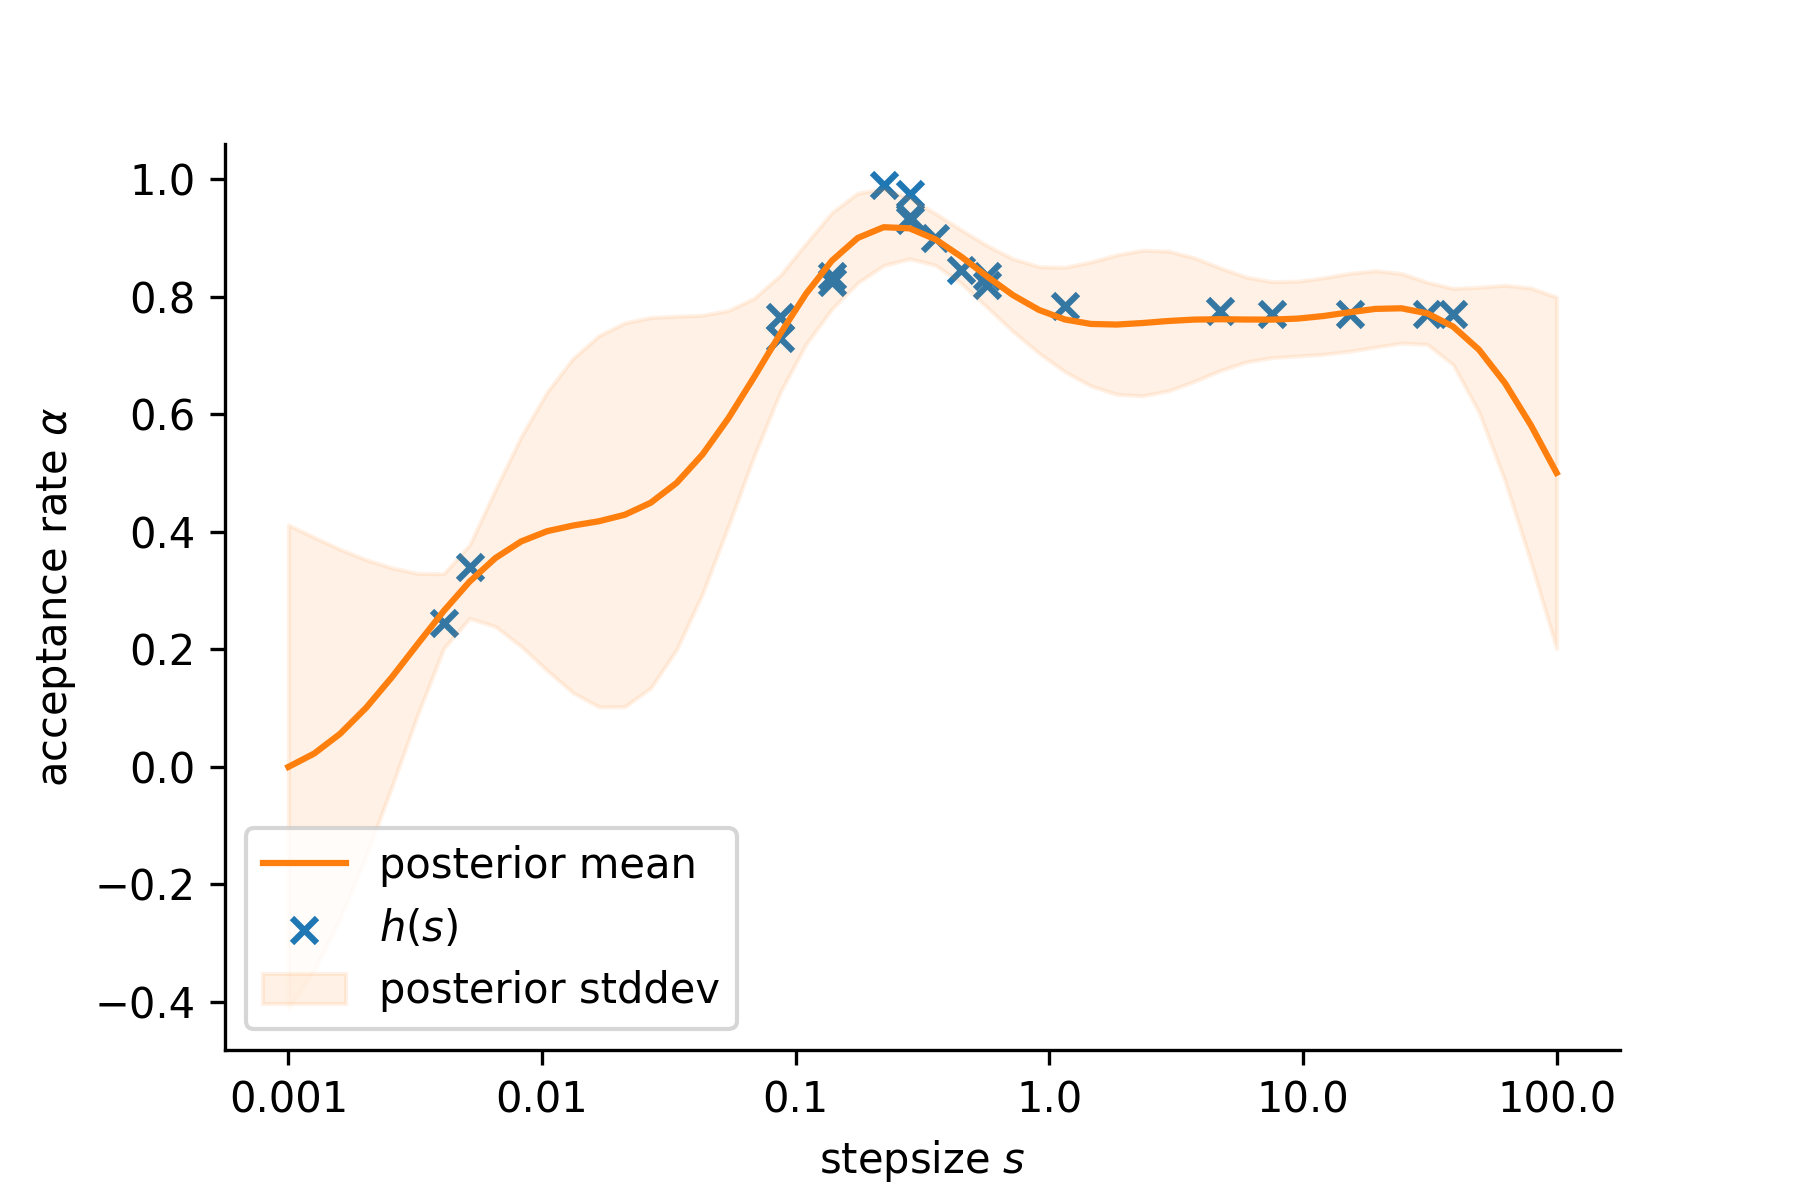
\includegraphics[scale=0.5]{imgs/accratethompsonsampling.png}
    \end{center}
    \vspace{-0.5cm}
\end{frame}

\begin{frame}[c]
    \frametitle{Agenda}
    \begin{itemize}
        {\color{lgray}
        \item Overwiew
        }
        \begin{itemize}
            {\color{lgray}
            \item Markov Chains \& Stepsizes
            \item Effectiveness \& Expected Squared Jump Distance 
            \item Thompson Sampling
            \item Once more: Why not to tune the acceptance rate!
            }
        \end{itemize}
        {\color{lgray}
        \item Results
        }
        \item Improvements \& More
        \begin{itemize}
            {\color{lgray}
            \item Acceptance Rate Tuning with Thompson Sampling
        }
            \item Tune higher-order Autocorrelation Lags
            {\color{lgray}
            \item Gaussian Process Time Costs
            \item Monotonicity of Thinning
        }
        \end{itemize}
    \end{itemize}
\end{frame}

\begin{frame}[c]
    \frametitle{Tune higher-order Autocorrelation Lags}
    \begin{itemize}
        \item Recap the definition $\mathrm{ESJD}(\theta) = \mathbb{E}[(\theta_{t+1} - \theta_t)^2]$ and observe, that
            \begin{align*}
                \mathbb{E}[(\theta_{t+k} - \theta_t)^2] = 
                &= \underbrace{\mathbb{E}[\theta_{t+k}^2]}_{=\mathbb{E}[\theta^2]} - 2\mathbb{E}[\theta_{t+k}\theta_t] + \underbrace{\mathbb{E}[\theta_t^2]}_{=\mathbb{E}[\theta^2]} \\
                &= 2\big(\mathbb{E}[\theta^2] - \mathbb{E}[\theta_{t+k}\theta_t]  + \mu^2 - \mu^2\big)\\
                &= 2\big(\sigma^2 - \big(\mathbb{E}[\theta_{t+k}\theta_t]  - \mu^2\big)\big)\\
                &= 2\sigma^2\big(1 - \frac{\mathbb{E}[\theta_{t+k}\theta_t]  - \mu^2}{\sigma^2}\big)\\
                &= 2\sigma^2\big(1 - \rho_k\big)\\
            \end{align*}
    \end{itemize}
\end{frame}

\begin{frame}[c]
    \frametitle{Tune higher-order Autocorrelation Lags}
    \begin{itemize}
        \item So we can minimize the lag-1 and lag-2 autocorrelation by maximizing the 1 and 2-jump ESJD:
            \begin{align*}
                \mathbb{E}[(\theta_{t+1} - \theta_t)^2] + \mathbb{E}[(\theta_{t+2} - \theta_t)^2] 
                &= 2\sigma^2\big(1 - \rho_1\big) +  2\sigma^2\big(1 - \rho_2\big)\\
                &= 2\sigma^2\big(2 - \rho_1 - \rho_2\big)\\
            \end{align*}
    \end{itemize}
\end{frame}

\begin{frame}[c]
    \frametitle{Agenda}
    \begin{itemize}
        {\color{lgray}
        \item Overwiew
        }
        \begin{itemize}
            {\color{lgray}
            \item Markov Chains \& Stepsizes
            \item Effectiveness \& Expected Squared Jump Distance 
            \item Thompson Sampling
            \item Once more: Why not to tune the acceptance rate!
            }
        \end{itemize}
        {\color{lgray}
        \item Results
        }
        \item Improvements \& More
        \begin{itemize}
            {\color{lgray}
            \item Acceptance Rate Tuning with Thompson Sampling
            \item Tune higher-order Autocorrelation Lags
            }
            \item Gaussian Process Time Costs
            {\color{lgray}
            \item Monotonicity of Thinning
            }
        \end{itemize}
    \end{itemize}
\end{frame}

\begin{frame}[c]
    \frametitle{Gaussian Process Time Costs}
    \begin{itemize}
        \item Recap Thompson Sampling:
            \begin{algorithm2e}[H]
                \For{$t \in 0, \ldots, m$}{
                    sample $\hat{f}_t \sim GP(\mu_t, \Sigma_t)$     \tcp*{$O(k(tc)^2)$ \phantom{$O(k)$ $O(cn)$ $O((tc)^3)$}} 
                    let $x_t := \mathrm{arg\,max} \, \hat{f}_t(x)$  \tcp*{$O(k)$ \phantom{$O(k(tc)^2)$ $O(cn)$ $O((tc)^3)$}} 
                    let $y_t := f(x_t)$                             \tcp*{$O(cn)$ \phantom{$O(k)$ $O(k(tc)^2)$ $O((tc)^3)$}} 
                    let $D_{t+1} := D_t \cup \{(x_t, y_t)\}$ \\
                    update $\mu_{t+1}$ using $D_{t+1}$              \tcp*{$O((tc)^3)$ \phantom{$O(k)$ $O(cn)$ $O(k(tc)^2)$}} 
                    update $\Sigma_{t+1}$ using $D_{t+1}$           \tcp*{$O((tc)^3)$ \phantom{$O(k)$ $O(cn)$ $O(k(tc)^2)$}} 
                }
            \end{algorithm2e}
            with $k = |X|$ the search grid, $n$ test samples, $c$ parallel chains and $m$ iterations rounds.
        \item Overall, we have $O((mc)^4)$\footnote[frame]{oof}
    \end{itemize}
\end{frame}

\begin{frame}[c]
    \frametitle{Agenda}
    \begin{itemize}
        {\color{lgray}
        \item Overwiew
        }
        \begin{itemize}
            {\color{lgray}
            \item Markov Chains \& Stepsizes
            \item Effectiveness \& Expected Squared Jump Distance 
            \item Thompson Sampling
            \item Once more: Why not to tune the acceptance rate!
            }
        \end{itemize}
        {\color{lgray}
        \item Results
        \item Improvements \& More
        }
        \begin{itemize}
            {\color{lgray}
            \item Acceptance Rate Tuning with Thompson Sampling
            \item Tune higher-order Autocorrelation Lags
            \item Gaussian Process Time Costs
            }
            \item Monotonicity of Thinning
        \end{itemize}
    \end{itemize}
\end{frame}

\begin{frame}[c]
    \frametitle{Monotonicity of Thinning}
    \begin{itemize}
        \item 
    \end{itemize}
\end{frame}

\begin{frame}[c]{}
    \centering
    \Huge \emph{Thanks!}
\end{frame}

